
%xhversion{v2.01 RdF} %PdJ,PdL,PdM,PdS,PdU,Pe6,PeI,PfB,PfD,RbN,RbP,RcL,RdC,RdD,RdF
%%%%%%%%%%%%%%%%%%%%%%%%%%%%%%%%%%%%%%%%%%%%%%%%%%%%%%%%%%%%%%%%%%%%%%%%%%%%%
%TODO: -siehe GitHub-Projects
%%%%%%%%%%%%%%%%%%%%%%%%%%%%%%%%%%%%%%%%%%%%%%%%%%%%%%%%%%%%%%%%%%%%%%%%%%%%%
%%%%
%	ifn="MeinLatexFile.tex"%%%%%%%%%%%%%%%%%%%%%%%%%%%%%%%%%%%%%%%%%%%%%%%%%%%%%%%%%%%%%%%%%%%%%%%%%
%	die auskommentierten 'usepackage'-Anweisungen sind
%	Alternativen oder Zusaetze, die iXH hier nicht,
%	aber vielleicht DU brauchen kannst - XH
%%%%%%%%%%%%%%%%%%%%%%%%%%%%%%%%%%%%%%%%%%%%%%%%%%%%%%%%%%%%%%%%%%%%%%%%%%%%%
%	XH Herstellungsprozess-Shellscript @15Apr17:
%	--------------------------------------------
%	#!/bin/sh
%	latex $ifn
%	fn2="$(echo $ifn|sed s/.tex/.dvi/)"
%	fn3="$(echo $ifn|sed s/.tex/-pics.pdf/)"
%	  ### now dvipdf  $fn2 into $fn3 Container ...
%	dvipdf $fn2  $fn3
%	#dvipdf $(echo $ifn|sed s/.tex/.dvi/)
%	  ### now pdflateXing $ifn ... (zweimal - fuers Inhaltsverzeichnis)
%	pdflatex $ifn
%	pdflatex $ifn
%\listfiles	
%%%%%%%%%%%%%%%%%%%%%%%%%%%%%%%%%%%%%%%%%%%%%%%%%%%%%%%%%%%%%%%%%%%%%%%%%%%%%
		%lists included files while processing 'pdflatex'
  %\documentclass[12pt,a4paper]{book}
  %\documentclass[11pt,a4paper]{article}
  %\documentclass[12pt,a4paper]{report}

  %\usepackage{etex}		%gegen 'no more room for new dimen...' error xh@RaE1

	% encoding:
  %%\usepackage[latin1]{inputenc}
  %%\usepackage[ansinew]{inputenc}
  %%\usepackage[cp850]{inputenc}
  %\usepackage[utf8x]{inputenc}  
\documentclass[12pt,a4paper]{article}
\usepackage[utf8]{inputenc}
\usepackage[T1]{fontenc}  %\usepackage{amssymb}
\usepackage{amsmath}
%\usepackage{extarrows}	%\xleftrightarrow[obentext]{untentext}
\usepackage{wasysym}
\usepackage{pxfonts}
\usepackage{verbatim}
\usepackage{alltt}
\usepackage{moreverb}
\usepackage{graphicx}
\usepackage{wrapfig}
%\usepackage{subfigure}\usepackage{hyperref}
\usepackage{nameref}
  %\usepackage{theorem}
  %\usepackage[dvips]{color}
  %\usepackage{lmodern}
  %\usepackage{textcomp}
\usepackage{multicol}		% 2-, 3-, ... -spaltige Formatierung mit 'multicols'
\usepackage{multirow}		% fuer 'tabular' - Tabellen
\usepackage{makeidx}
\usepackage{mdwlist}		% f. 'compact lists' "itemize*", "enumerate*", "description*"
  %\usepackage{ulem}	... produziertma nFehler ban 'latex' run
\usepackage{longtable}		% fuer tabellen ueber mehrere Seiten
\usepackage{xcolor}
\usepackage[ngerman]{babel}
\usepackage[pdfborderstyle={/S/U/W 1}]{hyperref}
\usepackage{float}
\usepackage{booktabs}
%\usepackage[demo]{graphicx}
%\addto{\captionsngerman}{%
  %\renewcommand*{\contentsname}{Inhaltsverzeichnis}
  %\renewcommand*{\listfigurename}{Abbildungen}
%  \renewcommand*{\listtablename}{Tabellen}
  %\renewcommand*{\figurename}{Abb.}
  %\renewcommand*{\tablename}{Tab.}
%}
%%%%%%%%%%%%%%%%%%%%%%%%%%%%%%%%%%%%%%%%%%%%%%%%%%%%%%%%%%%%%%%%%%%%%%%%%%%%%


\definecolor{lightgrey}	{gray}{0.85}
\definecolor{llltgy}	{gray}{0.98}
\definecolor{lltgy}	{gray}{0.96}
\definecolor{ltgy}	{gray}{0.91}
\definecolor{grey}	{gray}{0.75}
\definecolor{dkgy}	{gray}{0.35}
\definecolor{ddkgy}	{gray}{0.17}
\definecolor{dddkgy}	{gray}{0.07}
\definecolor{blk}	{gray}{0.99}
\definecolor{lltgn}	{rgb}{0.96,1.0,0.96}
\definecolor{ltgn}	{rgb}{0.91,1.0,0.91}
\definecolor{mdgn}	{rgb}{0.7,1.0,0.7}
\definecolor{dkgn}	{rgb}{0.0,0.7,0.0}
\definecolor{ddkgn}	{rgb}{0.0,0.45,0.0}
\definecolor{dddkgn}	{rgb}{0.0,0.25,0.0}
\definecolor{mdye}	{rgb}{0.95,0.95,0.60}
\definecolor{ltye}	{rgb}{0.98,0.98,0.90}
\definecolor{lltor}	{rgb}{0.97,0.94,.87}
\definecolor{ltor}	{rgb}{0.95,0.85,.66}
\definecolor{red}	{rgb}{1.0,0.0,0.0}
\definecolor{dkred}	{rgb}{0.8,0.0,0.0}
\definecolor{ltrd}	{rgb}{1.0,0.8,0.8}
\definecolor{ltbu}	{rgb}{0.8,0.8,1.0}
\definecolor{mdbu}	{rgb}{0.7,0.7,1.0}
\definecolor{bu}	{rgb}{0.0,0.0,1.0}
\definecolor{dkbu}	{rgb}{0.0,0.0,0.6}
\definecolor{ddkbu}	{rgb}{0.0,0.0,0.45}
\definecolor{ddkrd}	{rgb}{0.25,0.0,0.0}
\definecolor{dkrd}	{rgb}{0.70,0.0,0.0}
\definecolor{indigo}	{rgb}{0.2,0.1,0.9}

\usepackage{fancyhdr}
  %\usepackage{framed}		%'\begin{framed}' ... '\end{framed}', schautAusWiePartezettel:-)
\usepackage{hyphenat}		%fuer '\hyph{}'
  %\usepackage{lastpage}	%fuer '\pageref{LastPage}' - **funzt nid bei allen**
\usepackage{url}		%fuer '\url{...}'

% lscape oder pdflscape: ('landscape' == Querformat)
\usepackage{lscape}
  %\usepackage{pdflscape}
\usepackage{rotating}		%f. 'rotate' und 'turn'
\usepackage[active]{pst-pdf}
\usepackage{pst-circ}
\usepackage{pst-plot}
\usepackage{pst-uml}
  %\usepackage{calc}
\usepackage{fp}
\usepackage{pdfpages}
  %\usepackage[official]{eurosym}
\usepackage[gen]{eurosym}
\usepackage{acronym}
\usepackage[normalem]{ulem}
\useunder{\uline}{\ul}{}
	% YHs Raender links 30mm rechts 25mm einstellen:
\setlength{\hoffset}	{30mm-1in}
\setlength{\oddsidemargin}{0pt}		%bei doppelseitigem Druck umstellen!
\setlength{\textwidth}	{\paperwidth-55mm}

%hier duerfte header Fehler liegen
\setlength{\topmargin}	{0pt}
\addtolength{\voffset}  {-16.2mm}
\addtolength{\textheight}{39mm}

\setcounter{tocdepth}{4}		%bringt auch 'paragraph{titel}' ins Inhaltsverzeichnis

\newcommand{\cmnt}[1]{}			%eigene Kommentier-Funktion \cmnt{ ...Kommentar... }
\newcommand\tbs{\textbackslash}		%'\textbackslash{}' isma z'long zan tippen ;-)
\newcommand\dtbs{\textbackslash\textbackslash}	% -dito-
%
\definecolor{ydkbu}{rgb}{0.0,0.0,0.6}	% YHs blaue Schriftfarb
\newcommand{\yhbu}[0]{\color{ydkbu}}	% Macro fuer schreibfaulen XH
\definecolor{corrclr}{rgb}{0.7,0.2,0.2}		% XHs Korrekturen-Farb ...
\newcommand{\korr}[0]{\color{corrclr}\fontsize{8pt}{9pt}\selectfont\bf} %plus Faulheitsmacro
\makeindex

	%/* Line Spacing: */
\usepackage{setspace}
% \newcommand{\mylinespacing}[0]{\singlespace}
\newcommand{\mylinespacing}[0]{\onehalfspace}	% 1,5-ZeilenAbstand
% \newcommand{\mylinespacing}[0]{\doublespace}

% /*Font Family:*/
%\renewcommand*{\familydefault}{\rmdefault}	%klassisches 'Roman' (statt MicroMurx...)
\renewcommand*{\familydefault}{\sfdefault}	%klassisches 'Helvetica' statt 'MS-Arial'


%===================================================

\usepackage{listings}
\usepackage{color}
\newcommand*{\rom}[1]{\expandafter\@slowromancap\romannumeral #1@}

\definecolor{dkgreen}{rgb}{0,0.6,0}
\definecolor{gray}{rgb}{0.5,0.5,0.5}
\definecolor{mauve}{rgb}{0.58,0,0.82}

\lstset{frame=tb,
  language=Java,
  aboveskip=3mm,
  belowskip=3mm,
  showstringspaces=false,
  columns=flexible,
  basicstyle={\small\ttfamily},
  numbers=none,
  numberstyle=\tiny\color{gray},
  keywordstyle=\color{blue},
  commentstyle=\color{dkgreen},
  stringstyle=\color{mauve},
  breaklines=true,
  breakatwhitespace=true,
  tabsize=3
}

%===================================================
\begin{document}
%\addtocontents{toc}{\protect\begin{multicols}{2}} %-fuer mehrspaltiges Inh.Verz
%\lstset{language=German}



\newcommand\logoB[1]{%
	%dieses Macro '' zeichnet das "neue" HTL Logo mithilfe der
	% 'ps-tricks' Pakete/Anweisungen; Parameter#1 bestimmt die "Dicke"
	% der Balken; die "Groesse" bitte mit '\scalebox{factor}{logoB{0.12}}',
	% die Grundlinie mit '\raisebox{pos}{logoB{0.12}}' einstellen;
	% die Farbgebung spezifiziert man HIER:
  \definecolor{lobu}{rgb}{0.05,0.05,0.50}
  \definecolor{hibu}{rgb}{0.20,0.20,0.70}
  \definecolor{loye}{rgb}{0.85,0.75,0.36}
  \definecolor{hiye}{rgb}{0.99,0.92,0.00}
  \definecolor{logn}{rgb}{0.00,0.65,0.20}
  \definecolor{hign}{rgb}{0.00,0.79,0.30}
  \definecolor{lord}{rgb}{0.66,0.00,0.00}
  \definecolor{hird}{rgb}{0.89,0.00,0.00}%
  \resizebox{11.5mm}{!}{%
  \begin{pspicture}[showgrid=false](-1,-1)(1,1)
	\SpecialCoor	%das erlaubt PS -Berechnungen mit dem '!'; hier zur "DickenSkalierung"
	\pspolygon[linewidth=0.1pt,linestyle=none,fillcolor=lobu,fillstyle=solid]%
		(-#1, -1.00)( #1, -1.00)( 1.00, -#1)(! 1.00 #1 2 mul sub -#1)
	\pspolygon[linewidth=0.1pt,linestyle=none,fillcolor=hibu,fillstyle=solid]%
		(! 1.00 #1 2 mul sub          -#1)(! 1.00 #1 3 mul sub   0.00)%
		(! -#1         -1.00 #1 2 mul add)(-#1,-1.00)

	\pspolygon[linewidth=0.1pt,linestyle=none,fillcolor=hiye,fillstyle=solid]%
		( 1.00, -#1)( 1.00, #1)( #1, 1.00)(! #1   1.00 #1 2 mul sub)
	\pspolygon[linewidth=0.1pt,linestyle=none,fillcolor=loye,fillstyle=solid]%
		(! #1    1.00 #1 2 mul sub)(! 0.00   1.00 #1 3 mul sub)%
		(! 1.00 #1 2 mul sub   -#1)( 1.00, -#1)

	\pspolygon[linewidth=0.0pt,linestyle=none,fillcolor=hign,fillstyle=solid]%
		( #1, 1.00)( -#1, 1.00)(-1.00, #1)(! -1.00 #1 2 mul add   #1)
	\pspolygon[linewidth=0.0pt,linestyle=none,fillcolor=logn,fillstyle=solid]%
		(! -1.00 #1 2 mul add   #1)(! -1.00 #1 3 mul add    0.00)%
		(! #1    1.00 #1 2 mul sub)( #1, 1.00)

	\pspolygon[linewidth=0.1pt,linestyle=none,fillcolor=lord,fillstyle=solid]%
		(-1.00, #1)(-1.00, -#1)(-#1, -1.00)(! -#1    -1.00 #1 2 mul add)
	\pspolygon[linewidth=0.1pt,linestyle=none,fillcolor=hird,fillstyle=solid]%
		(! -#1   -1.00 #1 2 mul add)(! 0.00   -1.00 #1 3 mul add)%
		(! -1.00 #1 2 mul add    #1)(-1.00, #1)
	\NormalCoor
  \end{pspicture}%
  }%
}

\newcommand{\HtlHeader}[0]{%
	\hspace*{-11mm}%
	\raisebox{-1mm}{\logoB{0.12}}%
	\hspace*{2mm}%
	\parbox[b]{110mm}{\flushleft
		{\fontsize{20pt}{20pt}\selectfont\bf HTL}
		{\fontsize{16.2pt}{16.2pt}\selectfont\color{teal}\bf anichstrasse}
		\\[-4.05mm]{\color{darkgray}\rule{110mm}{0.5pt}}
		\\[-2.24mm]{\fontsize{7pt}{7pt}\selectfont\color{darkgray}
			Elektronik $\cdot$ Elektrotechnik $\cdot$
			Maschinenbau $\cdot$ Wirtschaftsingenieure
			\rule{0pt}{0mm}
		%\vspace*{1.1mm}
		}
	}%
	\hspace*{5mm}%
	\\[-1.5mm]\rule{\textwidth}{0.5pt}
	%\hfill
}%HtlHeader







	%/* Deckblatt */
\begin{titlepage}
 \begin{center}
   \begin{minipage}{\linewidth}
   \begin{center}
   \HtlHeader{}
	\vspace*{-10mm}
	{\fontsize{25pt}{25pt}\selectfont\bf \\[10mm]\text{DIPLOMARBEIT}}
	\\[19mm]{\fontsize{20pt}{20pt}\selectfont\textbf{\textsc{JavaChess, ChessPI AndChess}}}
	\\[15mm]{\fontsize{12.4pt}{12.4pt}\selectfont\bf
		Höhere Technische Bundeslehr- und Versuchsanstalt Anichstrasse}
	\\[ 5mm]\rule{132mm}{1.0pt}
	\\[ 4mm]{\fontsize{12.4pt}{12.4pt}\selectfont\bf Abteilung}
	\\[ 5mm]{\fontsize{12.4pt}{12.4pt}\selectfont\bf Elektronik \& Technische Informatik}
	\\[24mm]{\hspace*{2mm}\parbox{154mm}{\fontsize{12.4pt}{12.4pt}\selectfont
	  \parbox[t]{75mm}{
		Ausgeführt im Schuljahr 2017/18 von:
		\\[5.0mm]Alexander Beiser 5CHEL
		\\[2.5mm]Marcel Huber 5CHEL 
	  }
	  \hspace*{6mm}
	  \parbox[t]{50mm}{
		Betreuer/Betreuerin:
		\\[5.0mm]Ing. MSc. Signitzer Markus
	  }
	  \\[14mm]{Innsbruck, am 03.04.2018}
	  \\[16mm]\rule{150mm}{0.5pt}
	  \\[ 8mm]
	  \parbox[t]{75mm}{
		Abgabevermerk:
		\\[3.25mm]Datum:
	  }
	  \hspace*{6mm}
	  \parbox[t]{50mm}{
		Betreuer/in:
	  }
	}}
   \end{center}\hfill
   \end{minipage}
 \end{center}
\end{titlepage}


\addtocounter{page}{1}


%====================================================================================
%Liebe LaTeXniker!
%hierher kaeme das Inhaltsverzeichnis, empfehlenswerterweise mit Seitenwechsel
%\clearpage	%erzwingt Ausdruck noch ungedruckter 'floats'
%\vfill		%fuellt die Seite mit Leerraum auf
%\newpage	%erzwingt Seitenumbruch
%\tableofcontents
%====================================================================================

\renewcommand{\thepage}{\roman{page}}% Roman numerals for page counter
	%/*Header-Einstellung*/
\pagestyle{fancy}
\fancyhf{}
\renewcommand{\sectionmark}[1]{\markright{#1}}
\renewcommand{\subsectionmark}[1]{\markright{#1}}
\renewcommand{\subsubsectionmark}[1]{\markright{#1}}
\lhead{Diplomarbeit - JavaChess}
\chead{}
\rhead{Alexander Beiser, Marcel Huber}
\lfoot{5CHEL-2018}
\cfoot{\thesection-\rightmark}
%\cfoot{\thesubsubsection-\rightmark}
\rfoot[\thepage]{\thepage}
\setlength{\headwidth}	{1.0\textwidth}
\setlength{\headheight}{15mm}
\renewcommand{\headrulewidth}{0.0pt}
\renewcommand{\footrulewidth}{0.33pt}


\vfill
\newpage











%====================================================================================
%Best comment of all time!!!
\cmnt{
	Hier anfangs the Document Text.
	("\cmnt" isa self written very simple Macro for Kommentare:
	\newcommand{\cmnt}[1]{ }
                      !    !  !
                      !    !  +--- what to do, here also nix
                      !    +------ number of Parameters: se Kommentar-Text
                      +----------- name of new command
	)
	
	The "\yhbu" colored Sections are Vorgaben (recommendations) by AV YH.
	All se blue Zuig have to verschwind in se final version of your Diplomschrift(DS).
	(iXH recommend not to translate the words 'Diplomschrift' or 'Diplomarbeit'
	into 'diploma document', 'diploma project' or such Kas,
	because the original words are defined in se Austrian Law, Verordnungen
	and derlei rechtlix Plunder; so it is like an Eingenname,
	which we also dont uebersetz:
	You dont traslate 'HTL' to 'UTEC' (upper technical education corporation)
	or
	'Hansi' ('H', 'ans', 'i') 'Meier' ('M' and 'eier') into 'Ageoneeye Emeggs'
	oder?? )

	("\yhbu" Macro see above; is also a selber-defined macro:
	\definecolor{ydkbu}	{rgb}{0.0,0.0,0.5}   %make a Farb-Name
	               !          !     !   !   +--- Blau-Anteil
	               !          !     !   +------- Gruen-Anteil
	               !          !     +----------- Rot-Anteil
	               !          +----------------- Farbmodell 'RGB'
	               +---------------------------- name of se new Farb
	\newcommand{\yhbu}[0]{\color{ydkbu}}  %define se new macro
	              !    !       +--------- schreib des in LaTeX-Text eini
	              !    +----------------- 0 = null parameters, also keine
	              +---------------------- name of macro
	-> "\yhbu" gets replaced by "\color{ydkbu}"
	(what does this bring?:
	you can later change se color for all se "yhbu" parts gemeinsam
	without wurschtling through the whole document;
	also wenn mir die Farb no nid gfallt, aendris uanfoch in Macro)

	You can change the
		line spacing (einzeilig, 1.5zeilig und so)
	by schreibing one of
	   \newcommand{\mylinespacing}[0]{\singlespace}
	   \newcommand{\mylinespacing}[0]{\onehalfspace}
	   \newcommand{\mylinespacing}[0]{\doublespace}
	and using '\mylinespacing' in se document preamble (=header) part
	and the
		font family
		(Roman(serif) or se ugly Arial/Helvetica(sanserif))
	writing
	   \renewcommand*{\familydefault}{\rmdefault}
	   \renewcommand*{\familydefault}{\sfdefault}
	weiter oben in se preamble (isch bei se Macos oben)

	Be free to change se Deckblatt
	and se HTL-Header (dann isches aber nimma 'der HTL-Header'! ...and YH will fauch on you)

	mirXH persoenlich gfollaz besser min HTL-Header auf jedn Blattl
	(command: \lhead{\HtlHeader})
	he ghearat holt black-and-white, because colors gelten als 'kitschig' (kitchy)
	aber me asks jo nobody (i am only a small Wuerschtl from se behindmountain (Hintelgebilge))

	ATTENTION!
	This 'Inhaltsverzeichnis'
	does NOT pass zu se document text here.
	i just gewaltsam made it look like YH's Vorlage.
	iXH also dont understand,
	why it is mitten im Dokument anstatt at se beginnig or at se end,
	why se headline (Ueberschrift) is not at it's first page oben,
	but ganz lonely on the page before,
	and why it starts with Kapitel 2.1 anstatt 1.0
	and on page 8 statt 1 oder 2;
	it suggeriers that Loesungswege, Nutzwertanalysen, Grobwentwurf, Feinentwurf
	und Implementierung auf derselben Seite 11 Platz haben,
	Fertigungsdokumentation plus Gebrauchsanweisung (S.14)
	sowie das Pflichtenheft(S.18) nur 1 Seite lang sein brauchen,
	se p.22 must be empty
	and se Projektterminplanung erst am Ende des Projektes nach der
	Feststellung der Projekterfahrungen erfolgt.
	but i am eben a dumms kind, a small Wuerschtl...


}%cmnt
%====================================================================================

\mylinespacing
{




%====================================================================================
\newpage%\part{U-Lektionen \dq{}embedded Systems\dq{}}
%====================================================================================

\addcontentsline{toc}{section}{Erklärung der Eigenständigkeit der Arbeit}
\section*{\Large\sc Erklärung der Eigenständigkeit der Arbeit}
	\hfill\\[ 8mm]
	EIDESSTATTLICHE ERKLÄRUNG
	\\[3mm]
\begin{spacing}{1.5}
	\noindent%
	Ich erkläre an Eides statt, dass ich die vorliegende Diplomarbeit selbstaendig und
	ohne fremde Hilfe verfasst, andere als die angegebenen Quellen und Hilfsmittel
	nicht benutzt und die den benutzten Quellen wörtlich und inhaltlich entnommenen
	Stellen als solche erkenntlich gemacht habe.
\end{spacing}\hfill
	\\[12mm]
	\parbox[b]{52mm}{
		\rule{50mm}{0.2pt}\rule{0pt}{25mm}
		\\\hspace*{6mm}{Ort, Datum}
		\\[0mm]
	}
	\hfill
	\parbox[b]{72mm}{
		\rule{70mm}{0.2pt}\rule{0pt}{25mm}
		\\\hspace*{6mm}{Verfasser, Verfasserinnen}
		\\\hspace*{6mm}{Vor- und Zunamen}
	}







%======================================================================================
%\clearpage\vfill\newpage
%======================================================================================
\newpage
\section{Zusammenfassung des Projektergebnisses}
 \subsection{Kurzfassung /Abstract}
 
	Alexander Beiser und Marcel Huber entwickelten im Zuge ihrer Diplomarbeit 2017/18 ein Schachspiel, welches auf einem PC, Android-Smartphone und Raspberry PI spielbar ist. Das Schachspiel basierte auf einem bereits von ihnen geschriebenen rohen ,,Gerüst''. \\
	Dieses Spiel wurde mit der Programmiersprache Java entwickelt, weiteres war für den Raspberry PI ein Gehäuse zu designen und mit einem 3D Drucker zu realisieren. Um das Spielvergnügen für den Raspberry PI auch unterwegs zu ermöglichen, wurde eine Akkusteuerung entworfen und realisiert. \\
	\subsubsection{Alexander Beiser}
	Alexander Beiser war für große Teile des Backends zuständig. Ein Hauptteil bestand aus der Entwicklung einer Chess Engine, also eines Zündungsmechanismus, welcher speziell für die ebenso von Alexander Beiser erschaffene künstliche Intelligenz performiert wurde. Er entwickelte auch die Akkusteuerung für den Raspberry PI und designete das Gehäuse.
	
	\subsubsection{Marcel Huber}
	Marcel Huber war für weite Teile des Frontend Bereichs zuständig. Der Schwerpunkt lag auf dem Implementieren von JavaFX, dem Verbessern der audiovisuellen Gestaltung und dem Entwickeln eines Netzwerkspielmodus. Auch eine Andorid - app sollte entwickelt werden.
 
	\vfill
	\newpage	
	
 \subsection{Projektergebnis}
	{\yhbu
	Allgemeine Beschreibung, was vom Projektziel umgesetzt wurde, in einigen kurzen Sätzen.
	Optional Hinweise auf Erweiterungen.
	Gut machen sich in diesem Kapitel auch Bilder vom Gerät (HW) bzw. Screenshots (SW).
	\\[1mm]
	Liste aller im Pflichtenheft aufgeführten Anforderungen,
	die nur teilweise oder gar nicht umgesetzt wurden (mit Begründungen).
	}










%======================================================================================
\clearpage\vfill\newpage
%======================================================================================
\cmnt{	
	\vspace*{-10mm}\noindent%
	{\Large\bf Inhaltsverzeichnis}\\
 \renewcommand{\theenumii}{\arabic{enumii}}
 \renewcommand{\labelenumii}{\theenumi.\theenumii}
 \renewcommand{\theenumiii}{\arabic{enumiii}}
 \renewcommand{\labelenumiii}{\theenumi.\theenumii.\theenumiii}

{\yhbu
	Formale und sprachliche Aspekte \dotfill i		\\
	Zitierregeln \dotfill iv				\\
	Erklaerung der Eigenstaendigkeit der Arbeit \dotfill vii	\\
	Zusammenfassung des Projektergebnisses \dotfill viii		\\
	\phantom{11}Kurzfassung /Abstract \dotfill viii				\\
	\phantom{11}Projektergebnis \dotfill viii					\\
	1 Einleitung \dotfill 1					\\
	2 Vertiefende Aufgabenstellung \dotfill 1		\\
	\phantom{11}2.1 Schülername 1 \dotfill 1				\\
	\phantom{11}2.2 Schülerinnenname 2 \dotfill 1			\\
	3 Systemdokumentation \dotfill 2			\\
	\phantom{11}3.1 Lösungsweg \dotfill 2				\\
	\phantom{111}3.1.1 Gewählte Lösung \dotfill 2			\\
	\phantom{111}3.1.2 Alternative Lösungen (sollten Alternativen besprochen worden sein) \dotfill 2	\\
	\phantom{11}3.2 Grobentwurf \dotfill 2				\\
	\phantom{11}3.3 Feinentwurf \dotfill 2				\\
	\phantom{11}3.4 Implementierung \dotfill 2				\\
	\phantom{111}3.4.1 Sourcecode \dotfill 2				\\
	\phantom{111}3.4.2 Gesamtschaltplan und Fertigungsunterlagen \dotfill 3	\\
	\phantom{111}3.4.3 Verwendete Technologien und Entwicklungswerkzeuge \dotfill 3	\\
	\phantom{111}3.4.4 Testfälle \dotfill 4				\\
	\phantom{111}3.4.5 Test- und Messergebnisse \dotfill 4		\\
	4 Fertigungsdokumentation \dotfill 5			\\
	5 Benutzerdokumentation \dotfill 5			\\
	\phantom{11}5.1 Installationsanleitung \dotfill 5			\\
	\phantom{11}5.2 Anwendungsbeispiele \dotfill 5			\\
	\phantom{11}5.3 Referenzhandbuch \dotfill 5				\\
	\phantom{11}5.4 Fehlermeldungen und Hinweise auf Fehlerursachen \dotfill 5		\\
\clearpage\vfill\newpage{}\noindent%
	I. Abbildungsverzeichnis \dotfill I		\\
	II. Tabellenverzeichnis \dotfill I		\\
	III. Literaturverzeichnis \dotfill II		\\
	Anhang \dotfill IV				\\
	6 Pflichtenheft \dotfill IV			\\
	\phantom{11}6.1 Funktionale Anforderungen \dotfill IV	\\
	\phantom{11}6.2 Schnittstellen \dotfill IV			\\
	\phantom{11}6.3 Abnahmekriterien \dotfill IV		\\
	\phantom{11}6.4 Dokumentationsanforderungen \dotfill IV	\\
	\phantom{11}6.5 Qualitätsstandards \dotfill V		\\
	\phantom{11}6.6 Abwicklungsprozess \dotfill V		\\
	7 Zusammenfassung \dotfill VI			\\
	\phantom{11}7.1 Schlussfolgerung / Projekterfahrung \dotfill VI	\\
	\phantom{11}7.2 Projektterminplanung \dotfill VI		\\
	\phantom{11}7.3 Projektpersonalplanung und Kostenplanung \dotfill VII	\\
	\phantom{111}7.3.1 Projektkostenplan \dotfill VII		\\
	\phantom{111}7.3.2 Arbeitsnachweis Diplomarbeit \dotfill VII	\\
	\phantom{111}7.3.3 Leistungscontrolling \dotfill VII		\\
}
}	%



%=================================================================================
\clearpage\vfill\newpage{}
%=================================================================================

\section{Lizenz}
\label{SEC:licence}

Das Schachprogramm wird unter der ,,Creative Commons Attribution-NonCommercial-ShareAlike 4.0 International Public License'' entwickelt. \\
Dies räumt jeden Menschen folgende Rechte ein: 
\begin{itemize}
	\item{\textbf{Teilen:} Das Programm darf frei kopiert und weiterverteilt werden.}
	\item{\textbf{Verändern:} Das Programm darf frei verändert werden. Somit dürfen natürlich Verbesserungen implementiert werden.}
\end{itemize}

Allerdings muss dies unter den folgenden Bedingungen geschehen:
\begin{itemize}
	\item{\textbf{Zuschreibung:} Man muss die Namen der Entwickler entsprechend anführen und angeben, ob Veränderungen gemacht wurden.}
	\item{\textbf{Nicht kommerziell:} Das Programm darf nicht kommerziell benützt werden.}
	\item{\textbf{Gleiche Lizenz:} Sobald Veränderungen gemacht wurden, muss die Originallizenz weiter verwendet werden. Auch darf nicht von der obigen genannten Lizenz abgewichen werden.}
	\item{\textbf{Gesetzeskonform:} Das Programm darf nicht so verändert werden, dass die Nutzung illegal wird.}
\end{itemize}

\newpage
\section{Danksagung}
\label{SEC:THANKS}

Vor allem möchten wir unserem Betreuer Ing. MSc. Signitzer Markus für die Unterstüzung danken. \\
Weiters bedanken wir uns bei Fachlehrer Strohmaier für die Unterstüzung beim Bau des Gehäuses. \\[1ex]
Auch möchten wir uns bei Elektrotechnik Beiser - Andreas Beiser für die finanzielle Unterstüzung bedanken. \\[1ex]
Bei unserern Eltern, Brigitte und Andreas Beiser, bzw. bei Gabriele und Alexander Huber. \\
Die Bereitschaft unserer Beta-Tester unser Programm auf Herz und Nieren zu prüfen. \\
Weiteres wollen wir uns bei folgenden Personen Bedanken:
%\begin{itemize}
%	\item{\textbf{Raphael Meier} - Für die Unterstüzung beim Gehäusebau }
%	\item{\textbf{Chiara Polterauer (amtierende österreichische Schachmeisterin) %}- Für die Testung der KI}
%	\item
%	\item{\textbf{Brigitte Beiser} - Für das Korrekturlesen}
%	\item{\textbf{Alina Schärmer} - Für das Korrekturlesen}
%\end{itemize}


%=================================================================================
\clearpage\vfill\newpage{}
%=================================================================================

\tableofcontents


%=================================================================================
\clearpage\vfill\newpage{}
%=================================================================================
\renewcommand{\thepage}{\arabic{page}}% Arabic numerals for page counter
\setcounter{page}{1}
\setcounter{section}{0}
\section{\sc Einleitung}
\label{SEC:INTRODUCTION}

	Alexander Beiser und Marcel Huber sind beide begeisterte Schachspieler, womit die Entwicklung eines Schachspiels naheliegt. Gegen Ende des 4.Jahres der HTL trafen sie die Entscheidung ein Schachspiel selber zu entwickeln und keine Diplomarbeit von einer Firma anzunehmen. Für die Entwicklung ihres Schachspiels werden sie von ,,Elektrotechnik Beiser'' unterstützt. Diese Firma übernimmt die anfallenden Kosten für die Hardwarekomponenten.\\
	Anfang der 5.Klasse der HTL kamen die Sondierungsgespräche mit ihrem Betreuer Ing. MSc. Signitzer Markus, 
welcher ihnen bekannt gab, was im Zuge dieser Diplomarbeit alles erledigt werden muss. \\
Durch die Gespräche kam man zum Schluss, dass für die Diplomarbeit ein Schachspiel in Java entwickelt werden muss und dieses auf einen RaspberryPI, als auch auf Android Geräte potiert werden soll. Weiteres wird eine Akkusteuerung für den RaspberryPI entwickelt und ein Gehäuse designt und mittels schuleigenen 3D-Drucker ausgedruckt. \\
	Die GUI des Spiels soll mit JavaFX erstellt werden. Das Spiel soll gegen eine selbstentwickelte künstliche Intelligenz spielbar sein, im Hot Seat Modus oder im Local Area Network. \\
	Im Hot Seat Modus spielt man auf einem PC abwechselnd die Partien.
	Details werden in einem Pflichtenheft festgehalten, dieses Pflichtenheft befindet sich im Anhang.
	
\cmnt{
	{\yhbu
	In der Einleitung wird erklärt,
	wieso man sich für dieses Thema entschieden hat.
	(Zielsetzung und Aufgabenstellung des Gesamtprojekts,
	fachliches und wirtschaftliches Umfeld)
	}
	}
\section{\sc Vertiefende Aufgabenstellung}
 \subsection{Alexander Beiser}
 	Überarbeitung des Schachmattalgorithmus, Entwicklung der Zugmechanik und Entwicklung einer künstlichen Intelligenz. \\
Implementierung des Schachspiels auf den Raspberry-PI, gleichzeitige designen des Gehäuses für den Raspberry-PI und Entwicklung der Akkuansteuerungsschaltung. 
	
 \subsection{Marcel Huber}
	Entwicklung der Netzwerkfähigkeit und Implementierung von Java FX.
Verbesserung und Weiterentwicklung der audio- und visuellen Gestaltung.
Entwicklung der Android-App.


%=================================================================================
\clearpage\vfill\newpage{}
%=================================================================================

\section{Schach, eine Erklärung}
\label{SEC:CHESS}

\subsection{Was ist Schach?}
\label{SUBSEC:CHESS-EXPLAIN}
Um den Aufbau des Programmes nach vollziehen zu können, sollten die Grundregeln des Schachspiels geläufig sein. Hier haben wir versucht, die wichtigsten Regeln kurz zusammenzufassen. \\
Was ist Schach? \\
Schach ist ein strategisches Brettspiel, indem es darum geht, die feindliche Seite zu schlagen. Die feindliche Seite hat verloren, wenn der König im Schachmatt steht. \\
Der Name Schach kommt aus dem persichen ,,Schah'' und bedeutet so viel wie König, woher der Name ,,königliches Spiel'' stammt. \\
Ursprünglich wurde das Spiel vermutlich in Nordindien erfunden und kam im Zuge der islamischen Expansion, von 630 bis ca. 750, nach Europa \cite{wiki:chess}.


\subsection{Spielregeln}
\label{SUBSEC:GAMERULES}

Nach der ersten Erklärung, was Schach ist, kommen wir zu den Spielregeln.
Schach wird auf einem 8*8 karierten Feld gespielt. Die Nummerierung erfolgt horizontal durch das Alphabet, a bis h und vertikal durch Ziffern, 1 bis 8.
Zu Beginn gibt es zwei Teams, meist Weiß und Schwarz, mit jeweils 16 Figuren.
Folgende Figuren sind zu Beginn am Feld:
\begin{itemize}
	\item{8 Bauern}
	\item{2 Springer}
	\item{2 Läufer}
	\item{2 Türme}
	\item{1 Dame}
	\item{1 König}
\end{itemize}

Das Ende des Spiels erfolgt entweder durch schachmatt, Aufgabe oder durch ein Remis/Patt. Schachmatt bedeutet, dass der König bedroht wird und es dem Spieler nicht mehr möglich ist den König aus dieser Position zu befreien.
Patt Möglichkeiten:
\begin{itemize}
	\item{ entsteht, wenn eine der Parteien keinen legalen Zug mehr ausführen kann }
	\item{Durch ein ,,technisches Remis'', wenn außer den beiden Königen nur mehr ein Läufer oder Springer am Feld ist.}
	\item{Wenn 50 Züge lang keine Spielfigur geschlagen oder kein Bauer bewegt wurde und der am Zug befindliche Spieler das Remis verkündet.}
	\item{Wenn eine identische Stellung drei Mal mit identischen Zugmöglichkeiten mindestens drei Mal vorkommt, kann ein Spieler ein Remis beantragen.}
\end{itemize}

Nun folgen die Zugregeln:

\subsubsection{Zugregel Bauer}
\label{SUBSUBSEC:PAWN}
\begin{itemize}
	\item{Bauer darf einen Schritt nach vorne ziehen, wenn das Feld leer ist}
	\item{Befindet sich der Bauer in der Ausgangsposition und wurde noch nicht gezogen, kann er auch wahlweise zwei Schritte vorrücken.}
	\item{Der Bauer schlägt vorwärts diagonal ein Feld.}
	\item{Spezialzug: ,,En Passant''. Dies kann er als einzige Spielfigur, wenn ein feindlicher Bauer zuvor einen Doppelschritt gemacht hat und somit den eigenen Bauern die Option nimmt, den gegnerischen Bauern anzugreifen. Falls er ausgeführt wird, ist der feindliche Bauer vernichtet und der eigene rückt diagonal ein Feld hinter den nicht mehr existierenden Bauern.}
	\item{Sobald ein Bauer die gegnerische ,,Grundreihe'' erreicht, wird ein Bauerntausch durchgeführt. Hier muss der Bauer gegen eine Dame eingetauscht werden.}
\end{itemize}

\subsubsection{Zugregel Springer}
\label{SUBSUBSEC:JUMPER}
\begin{itemize}
	\item{Der Springer darf auf das Feld ziehen, dass zwei Felder horizontal bzw. diagonal und eines diagonal bzw. horizontal (gegengleich) versetzt ist. z.B.: Von  b8 auf c6}
\end{itemize}
\subsubsection{Zugregel Läufer}
\label{SUBSUBSEC:BISHOP}
\begin{itemize}
	\item{Läufer dürfen diagonal, so weit wie sie wollen ziehen und schlagen, jedoch darf er nicht über eine Figur ziehen.}
\end{itemize}

\subsubsection{Zugregel Turm}
\label{SUBSUBSEC:ROOK}
\begin{itemize}
	\item{Ein Turm darf horizontal bzw. vertikal ziehen und schlagen wie weit er will, jedoch nicht über Figuren hinweg.}
\end{itemize}

\subsubsection{Zugregel Dame}
\label{SUBSUBSEC:QUEEN}
\begin{itemize}
	\item{Eine Dame darf horizontal, vertikal bzw. diagonal ziehen und schlagen so weit wie sie will, jedoch nicht über Figuren hinweg.}
\end{itemize}

\subsubsection{Zugregel König}
\label{SUBSUBSEC:KING}
\begin{itemize}
	\item{Der König kann horizontal, vertikal bzw. diagonal ein Feld ziehen.}
	\item{Spezialzug: ,,Rochade''. Dabei wird der König entweder zwei Felder nach links, bzw. zwei Felder nach rechts bewegt. Der Turm bewegt sich dabei drei Felder nach rechts bzw. zwei Felder nach links. König und Turm dürfen bis zu diesem Zug noch nicht bewegt worden sein, weiters darf keines der Felder über das sie ziehen, der König oder der Turm bedroht werden.}
\end{itemize}


%===========================================================================================

\subsection{Schachmaschinen}
\label{SUBSUBSEC:CHESS-COMPUTERS}

Seitdem es die Möglichkeit gibt einen Schach spielenden Mechanismus zu bauen, hat man dies auch getan. Zu Anfang war dies noch der ,,Schach spielende Türke'', welcher 1769 von Wolfgang von Kempelen konstruiert wurde. \\ 
Der richtige Durchbruch geschah aber erst durch die Erfindung des Computers. Die Hardware wurde immer Leistungsfähiger, wodurch der Mensch als Gegner immer weiter in Bedrängung geriet. 1997 schlug der von IBM speziell entwickelte Schachcomputer Deep Blue, den damaligen Schachweltmeister Kasparow, wodurch die Künstliche Intelligenz in diesem Bereich offiziell den Menschen überholt hat. \\
Heutzutage wird gegen Schachcomputer vor allem zu Trainingszwecken gespielt. Solche Schachcomputer finden sich mittlerweile auf so ziemlich jedem Gerät, egal ob Smartphone, Tablet oder PC/Laptop. Meist sind diese Programme aber Proprietär und ,,closed source''. Wir entwickeln deshalb ein ,,open Source'' Schachspiel, dass auf mehreren Devices spielbar ist.
 



 
%===========================================================================================
\clearpage\vfill\newpage{}
%===========================================================================================

\section{Java Chess}
\label{SEC:JAVACHESS}

\subsection{Einführung}
\label{SUBSEC:JAVACHESS-INTRO}

Bevor mit der Dokumentation des Programmcodes begonnen werden kann, werden zuerst einige Möglichkeiten beschrieben, wie ein Schachprogramm prinzipiell programmiert werden kann.

Hierfür gibt es prinzipiell zwei Möglichkeiten:
\begin{enumerate}
	\item{Die Figuren kennen ihre Position}
	\item{Das Brett kennt die Positionen der Figuren}
\end{enumerate}

Das die Figuren ihre Position kennen, klingt zuerst gar nicht so abwegig. Probleme treten aber auf, sobald schachmatt überprüft werden soll. Hierfür muss überprüft werden, ob irgendeine gegnerische Figur den König schlagen kann, wofür man aber das Objekt der Figur benötigt. Natürlich ist dies Programmiertechnisch kein Problem, dadurch entstehen aber längere Wartezeiten. 


Falls das Brett die Position der Figuren kennt und diese Figuren lediglich über eine Zahlenmatrix dargestellt werden, ist das Spiel nicht nur sehr viel performanter, es ergeben sich auch große Vorteile beim Entwickeln der künstlichen Intelligenz. \\ 
Wir entschieden uns für diese Lösung.

\subsection{Java Chess - Übersicht}
\label{SUBSEC:JAVACHESS-OVERVIEW}

JavaChess ist in der Programmiersprache Java geschrieben. Java ist eine Objektorientierte, Klassenbasierte Hochsprache der Informatik. Java hat den Vorteil, dass es nicht Hardware gebunden ist und somit ein Programm, geschrieben auf einer Distribution des Betriebssystems GNU/Linux auf (zumindest theoretisch) allen unterstützten Systemen läuft. \\
Somit können wir unser Spiel auch auf einem Raspberry-PI lauffähig machen. \\
Das von uns verwendete \acl{GUI} Environment ist JavaFX. Es wurde erstmals im Dezember 2008 den Programmierern zugänglich gemacht und soll das bis dahin Standard Java GUI Environment ,,Swing'' ersetzen. Die Unterschiede bestehen im Aufbau, wie eine GUI realisiert werden kann bis hin zu den verbesserten grafischen Effekten, die durch JavaFX möglich sind. \\

Dadurch wurden die Entscheidungen gefällt Java mit JavaFX zu verwenden.\\
Java Chess nützt in Folge einige dieser Vorteile aus, vor allem Objektorientiertes Design. 


\subsubsection{Blockschaltbild}
\label{SUBSUBSEC:BLOCKSCHALTBILD}

Hier wird ein Einblick gegeben, wie Java Chess funktioniert. Dies geschieht anhand von einem Blockschaltbild, welches Pakete bzw. Klassen beschreibt: \\
\vspace{1cm}


\begin{figure}[H]
  \centering
   	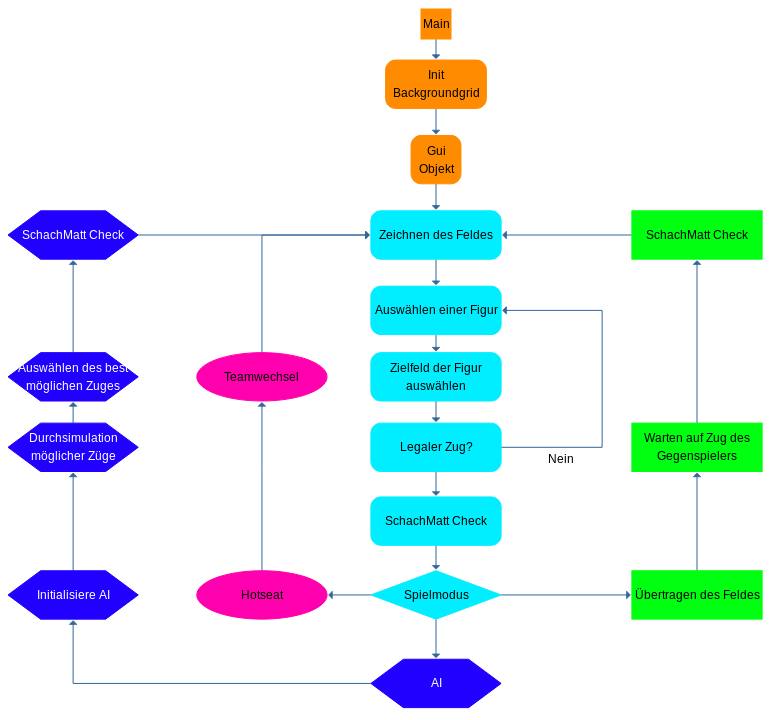
\includegraphics[width=14cm]{graphics/block.png}
  \caption{Das Blockschaltbild}
  \label{fig:block}
\end{figure}

\subsection{Package- und Klassenübersicht}
\label{SUBSEC:PACKAGE}

Im folgenden werden die groben Inhalte und Funktionen der Packages und Klassen zusammengefasst.\

\subsubsection{audio}

Dieses Package beinhaltet alle Klassen, die benötigt werden, um die Soundeffekte im Spiel abzuspielen. Zusätzlich sind die benötigten Audiofiles enthalten.\

\begin{itemize}
	\item{\textbf{AudioManager.java}: Diese Klasse Managed die zwei Möglichkeiten, Audiodateien im Programm abzuspielen. Warum dies notwendig ist, wird in der entsprechenden Sektion erklärt. %TODO
Auch die Einstellungsvariablen für die Sounds (z.B. Lautstärke) werden hier gespeichert. }
	
	\item{\textbf{JavaFxAudio.Java}: Mit dieser Klasse werden die Sounds für den JavaFX - Soundplayer geladen und abgespielt. }	
	
	\item{\textbf{NativeAudio.java}: Dies Klasse wurde nachträglich hinzugefügt und ermöglicht das Abspielen von Sounds auf Systemen, welche den JavaFX-Soundplayer nicht unterstützen.}
	
\end{itemize}

\subsubsection{backgroundmatrix}

In diesesm Package sind Klassen beheimatet, die für die Spiellogik verantwortlich sind.

\begin{itemize}
	\item{\textbf{BackgroundGrid.java}: Dies ist eine 'Basisklasse' der Spiellogik. In ihr werden Schach- und Schachmattabfagen durchgeführt. Zusätzlich werden in ihr verschiedene Spielrelevante variablen gespeichert, beispielsweise das aktuell ziehende Team.}
	
	\item{\textbf{Move.java}: In dieser Klasse werden die Erlaubten Zugmuster für jede einzelne Figur vermerkt und ausgewertet.  }

\end{itemize}
 
\subsubsection{game}

Die Klassen für die einzelnen Spielmodi werden in diesem Package abgelegt. 


\begin{itemize}

	\item{\textbf{AI}: Ist quasi Schnittstelle zwischen AILogic und restlichem Spiel. Wird als neuer Thread gestartet, um das restliche Spiel nicht zu beeinflussen. Ruft AILogic auf.}
	
	\item{\textbf{AILogic}: Hier ist der eigentliche KI-Algorithmus. Wertet alle möglichen Züge nach dem Bestmöglichen aus.}

	\item{\textbf{AIvsAI.java}: Diese Klasse reguliert den 'geheimen Spielmodus', in dem der Computer gegen sich selbst spielt. }
	
	\item{\textbf{LAN.java}: In dieser Klasse werden alle Variablen für den LAN-Spielmodus gespeichert. Zudem werden die Schnittstellen zur Netzwerkkommunikation bereitgestellt.}
	
	\item{\textbf{Local.java}: Diese Klasse beinhaltet die Variablen für den Lokalen Modus. }

	\item{\textbf{MovePos.java}: Dies Klasse stellt eine Hilfsklasse dar. Sie wird benutzt, um die momentane, zukünftige, vergangene oder spezial Position von Figuren zu bestimmen.}

\end{itemize}

\subsubsection{gui}

In diesem Package sind alle Klassen zusammengefasst, die etwas mit der GUI, also mit dem 'Graphical User Interface' zu tun haben. 

\begin{itemize}

	\item{\textbf{About.java}: Diese Klasse generiert ein Popup, welches auskunft über die Entwickler und die Lizenz gibt. }
	
	\item{\textbf{BoardGui.java}: In dieser Klasse wird das Schachbrett gezeichnet. Außerdem werden hier usereingaben mit der Maus verarbeitet und es werden grafische Effekte erzeugt. Auch wird in dieser Klasse ein Teil des Spielflussess, insbesondere das Senden und Empfangen des Lan-Modus, geregelt. }
	
	\item{\textbf{GUI.java}: Diese Klasse erweitert die FX - Applikationsklasse. Sie stellt alle graphischen Elemente dar und regelt deren Platzbedarf. Manche Funktionen, wie beispielsweise das starten eines neuen Spiels oder das Laden eines Spielfeldes, sind hier enthalten }
	
	\item{\textbf{Help.java}: Die Helpklasse erzeugt ein Popup, in welchem die Spielanleitung angezeigt wird.}
	
	\item{\textbf{Menu.java}: Die Menüklasse erzeugt das Spielmenü. Alle Funktionen aus dem Menü werden hier ausgeführt oder zumindest aufgerufen. Konkreet werden Spielmodi gewechselt, Felder gespeichert oder geladen, neue Spiele gestartet und es werden die Popups aufgerufen.}
	
	\item{\textbf{Popup.java}: Diese Klasse erzeugt ein Popup, in dem viele Spielelemente konfiguriert werden können. Genauer werden die Lautstärke, AI-Schwierigkeit, und weitere kleine Einstellungen angeboten. Zusätzlich werden Informationen zum Spiel angezeigt. }
	
	\item{\textbf{Tile.java}: Dies Klasse repräsentiert ein Feld auf dem Schachbrett und enthält dessen Informationen.}

\end{itemize}

\subsubsection{images}

Dieses Package enthält alle Bilddateien die benötigt werden, um das Spielfeld darzustellen. 

\subsubsection{launchpad}

In diesem Package sind alle Klassen beinhaltet, welche den Launchpad-Support ermöglichen. 

%TODO Launchpad-Doku

\subsubsection{network}

Dieses Package beinhaltet alle Klassen, die benötigt werden, um dan Netzwerkspielmodus zu ermöglchen.

\begin{itemize}
	\item{\textbf{Heartbeat.java}: Diese Klasse stellt sicher, dass der Verlust einer Netzwerkverbindung erkannt wird.}
	\item{\textbf{hostingJob.java}: Diese Klasse wird benötigt, um das Hosten eines Netzwerkspieles zu regeln. Genaueres dazu unter} %TODO
	\item{\textbf{ReadingJob.java}: Dies Klasse ermöglicht es, Objekte vom Netzwerk zu empfangen. }
\end{itemize}

\subsubsection{saveload}

\begin{itemize}

	\item{\textbf{Load.java}: Diese Klasse enthält alle notwendigen Funktionen, um Spielstände zu laden. Außerdem werden alle Fehler, die beim Ladevorgang auftreten können, hier bearbeitet.  }
	
	\item{\textbf{Save.java}: Um Spielstände zu speichern wird diese Klasse benötzigt. Sie enthält alle notwendige Funktionen dazu, und bearbeitet Fehler, die beim Speichern auftreten können. }


\end{itemize}

\subsubsection{start}

Dieses Package entält die Klasse '\textit{Main.java}', welche nur dazu dient, das Spiel zu starten.

\newpage
\subsection{Initialisierung}
\label{SUBSEC:INIT}

\cmnt{Hier soll erklärt werden wie JavaChess initialisiert wird.}

Als Referenz bzw. Hilfe siehe \ref{SUBSUBSEC:BLOCKSCHALTBILD}.
Zuerst startet das Programm in der Main Methode der Main Klasse. Als Nächstes wird das Backgroundgrid Objekt initialisiert und das GUI-Objekt von der GUI-Klasse geladen. \\
Dieses Objekt ladet im Anschluss die Board Gui Klasse, welche ein Canvas ist. In diesem ist eine gewisse Art des Zeichnens möglich. Dadurch wird auch das Schachbrett gezeichnet und in dieser Klasse findet der ,,Spielfluss'' statt. \\ 
Im Default Modus startet das Spiel im ,,Hot-Seat" game mode, siehe \ref{SUBSEC:LOCAL_MODE}. Hier spielt der Spieler zuerst einen Zug, woraufhin kontrolliert wird, ob der Zug legal ist. Da das Spiel im Hot-Seat-Mode startet, wechselt der Spieler und das Schachbrett wird mit der Aufstellung nach Zug 1 neu gezeichnet.

\subsection{Repräsentation der Figuren:}

Die Figuren werden über eine Zahlenmatrix repräsentiert. Dabei bekommt jede Figur eine individuelle Zahl zugeteilt. \\
Eine solche Zahl besteht aus drei Ziffern, z.B.: 102. Diese ist der 2. weiße Bauer, die 1. Ziffer gibt dabei an, ob es Team Weiß (1) oder Schwarz (2) ist. Die 2. Ziffer gibt den Figurentyp an, also Bauer, Turm, etc. Die 3.Ziffer gibt an die wievielte Figur es ist. \\
Diese Matrix ist in einem Objekt von der ,,Background-Matrix'' gespeichert. \\
Zu Beginn einer jeden Partie wird einmal die Startaufstellung im ,,Constructor'' der ,,Background-Matrix'' initialisiert:

	\begin{table}[H]
		\centering
		\begin{tabular}{| c | c | c | c | c | c | c | c |}
			\hline
			110 & 120 	& 	130 & 140 	& 150 	& 131 	& 121 	& 	111 \\ \hline
			101 & 102 	& 	103 & 	104 & 	105 & 	106 & 	107 & 	108 \\ \hline
			0	&	0	& 	0	&	0	&	0	&	0	&	0	&	0	\\ \hline
			0	&	0	& 	0	&	0	&	0	&	0	&	0	&	0 	\\ \hline
			0	&	0	& 	0	&	0	&	0	&	0	&	0	&	0 	\\ \hline
			0	&	0	& 	0	&	0	&	0	&	0	&	0	&	0 	\\ \hline
			201 &	202 &	203	&	204	&	205	&	206	&	207	&	208	\\ \hline
			210 & 	220	&	230	&	240	&	250	&	231	&	221	&	211 \\ 
			\hline	
		\end{tabular}
		\caption{Repräsentation der Figuren}
		\label{TABLE:REPRESENTATION-MEEPLES}
	\end{table}

Durch diese Matrix werden in Folge alle Zugberechnungen, KI-Berechnungen, etc. durchgeführt. \\


\subsection{Zugmechanik und Local-Mode}
\label{SUBSEC:LOCAL_MODE}

Sobald das Spiel geladen und initialisiert ist, wird automatisch der Hot-Seat Spielmodus ausgewählt. Beim Hotseat Modus spielt man auf einem Device nacheinander. Dieses eigentliche Spiel geschieht in einem Objekt der ,,BoardGui'' Klasse. Die BoardGui Klasse ist ein Canvas Objekt, also ein Objekt, auf dem man zum Beispiel zeichnen kann. Diese Funktion wird ausgenutzt, um das Spielfeld zu zeichnen. Wie dies genau geschieht wird in \textbf{ %TODO
 } 
erläutert.  \\
Nun ist der weiße Spieler an der Reihe. Welches Team an der Reihe ist, wird durch den Boolean ,,team'' bestimmt. Dieser Spielstand wird in einem Objekt der Backgroundgrid Klasse gespeichert. True bedeutet, dass der weiße Spieler am Zug ist, false das der Schwarze am Zug ist. \\
Der Spieler kann nun die Figur anwählen, die er bewegen möchte, oder die linke Maustaste gedrückt halten und so die Figur über das Brett ,,schweben'' lassen. In dieser Position werden alle möglichen Bewegungen des Spielsteins angezeigt. Hier ist zu erwähnen, dass potenzielle Angriffe anders dargestellt werden, wie eine Bewegung. \\
Nun muss der Spieler nur noch das Feld, auf das er ziehen möchte, klicken bzw. die Figur darüber absetzen. Der Move Algorithmus berechnet nun, ob dieser Zug auch möglich ist. Falls dieser Zug erlaubt ist, wird die Hintergrundmatrix entsprechend umgeschrieben, entsprechend den neuen Positionen der Figuren. \\
Im Hotseat mode wird jetzt das Team gewechselt und die GUI neu gezeichnet, damit die Änderungen in der Matrix sichtbar werden. 

\subsubsection{Die Move Klasse - Funktion}
\label{SUBSUBSEC:MOVE}

Es gibt aber mehrere Möglichkeiten, wie eine Abfrage des erlaubten Zuges entwickelt werden kann. Der 1.Ansatz bestand darin, dass jede Figur ihren erlaubten Zug selber überprüft. Hierbei muss klar sein, dass wir für jede Figur ein eigenes Objekt, des jeweiligen Klassentypes (z.B.: Bauer) angelegt haben. Für die Zugüberprüfung wird an die Figur die Position übergeben, wohin sie ziehen soll und das momentane Spielfeld. Ein Boolean als Rückgabewert hat dann indiziert, ob dieser Zug legal war. \\
Bevor eine solche Move-Abfrage, aber überhaupt durchgeführt werden kann, muss diese auch aufgerufen werden und erkannt werden, welcher Spielstein ausgewählt wurde. Dies geschah über eine weitere Move Klasse
Der 1. Ansatz war somit nicht wirklich eine Klasse, sondern auf viele Klassen verteilt. Funktioniert hat dies ohne bekannte Bugs, dadurch ist der Code aber stellenweise sehr unübersichtlich geworden. Das Spiel wurde teilweise nicht performant und eine AI mit diesem Ansatz zu schreiben ist schlicht unvorstellbar. \\[2ex]
Der 2. Ansatz bestand darin, alle Zugabfragen in einer Klasse zu implementieren. Dazu wurde dem Objekt dieser Klasse, die Koordinaten des zu bewegenden Spielsteines gegeben, wo dieser ist und wohin gezogen werden soll und das Spielfeld. Geprüft wird wieder, ob der Spielzug erlaubt ist. Auch geschieht die Abfrage, welcher Spielstein ausgewählt wurde wieder über eine extra Klasse.\\ 
Vorteile ergeben sich aus der Übersicht, das Problem mit der Performance hat sich auch weitestgehend gelöst. Das Problem mit der KI ist aber geblieben und nun ist ein weiteres Problem dazugekommen: Wenn man auf eine Figur klickt, erscheinen alle Felder, auf die man ziehen kann. Dies ist mit dieser Implementierung der Move Klasse wiederum eine Unmöglichkeit zu programmieren.\\[2ex]
Der 3.Ansatz beschäftigt sich mit der Vorschau der möglichen Züge. Man gibt dem Objekt der Move Klasse einfach alles, was bereits im 2. Ansatz übergeben wurde. Nun wird aber ein int[][] aus möglichen Zügen zurückgegeben. Dies funktionierte ohne Probleme. \\
Das Einzige was als Problem deklariert werden kann, ist das dadurch das ,,DRY'' (Don't repeat yourself) Prinzip verletzt wurde. In der Move Klasse gab es nun einmal die Abfrage, ob der Zug erlaubt ist und einmal die Abfrage, welche Züge erlaubt sind. Für die KI ist es von Vorteil, wenn sie alle möglichen Züge eines Spielsteines bekommt. Es sollte aber auch klar sein, welcher Spielstein zuvor auf dem Feld stand, was durch diese Methode nur indirekt möglich ist. \\[2ex]
Der 4.Ansatz nimmt sich allen diesen Problemen an, indem den 3. Ansatz ausbaut und eine neue ,,MovePos'' Klasse einführt. Die Move-Klasse kann nun als eine Art Box verstanden werden: Man sagt der Move Methode, welche Figur man ausgewählt hat und man erhält alle möglichen Züge als MovePos-ArrayList zurück. Der eigentliche Zug muss aber extern durchgeführt werden. \\
Das Objekt der Klasse MovePos, beinhaltet die alte Position des Spielsteins, die neue Position, die ID des Spielsteins, die ID des Feldes auf das gezogen wurde und für die Rochade bzw. den En-Passant noch zwei weitere Informationen zu den Feldern, wo und was darauf war. \\
Dadurch wird für die KI-Berechnung, für die Zugüberprüfung und für das Anzeigen aller möglichen Züge die gleiche Basisstruktur der Zugberechnung verwendet. Der Unterschied besteht darin, dass die KI direkt die Zugberechnung aufruft, währenddessen die Zugüberprüfung und das Anzeigen der möglichen Züge auf die Methode GetMove zurückgreift (überschreiben das Spielfeld).\\


\subsubsection{Die Move Klasse - Code}
\label{SUBSUBSEC:MOVECODE}


Die Move Klasse beinhaltet momentan ca. 1400 Zeilen Code. \\
Die folgende Dokumentation erfolgt als Pseudo Code:

\lstset{language=Java}
\begin{lstlisting}
import...
...
public class Move{
	private ArrayList _HitList;
	private ArrayList _MoveList;
	private ArrayList _LastMoveList;
	private boolean _bSelect;
	private int _iSelect;
	...
	public Move(){
		_bSelect = false;
		...
		das Standardmaessig keine Figur ausgewaeht wurde
		...
	}			
	...
	//Methode fuer Spielerzug bzw. zum anzeigen aller moeglichen Positionen
	public int[][] GetMove(Position und ID von Spielfigur, Objekt von Hintergrundmatrix){
		...
		//Die Differenz zwischen zuvor ausgewaehlter Figur und jetzt ausgewaehlten Zug Feld		
		iDif = iPos - _iSelect
		//Wenn die Figur bewegt werden darf
		if(_bSelect && iDif >= 50){
			//ArrayList von der Klasse MovePos
			ArrayList MoveList = getMoveMeeple(Spielfeld,Team, Position Figur)
			for(MovePos MP in MoveList){
				if(MP-Position == Gewaehlte Position){
					...
					Ueberschreiben des alten Feldes mit den neuen Positionen
					Auch fuer alle Spezialzuege
					...		
				}
				
			}
		} else {
			...
			alle moeglichen Zuege
			...
			if(Position ist Figur){
				ArrayList MoveList = getMoveMeeple(Spielfeld,Team,Position Figur)
				for(MovePos MP in MoveList){
					if(Zug auf Leeres Feld){
						_MoveList.add(GezogenesFeld)
					}else{
						_HitList.add(GezogenesFeld)
					}
				}
			}
		}	
		return GeaendertesSpielfeld		
	}
	
	//Herzstueck der Move Klasse - gibt alle moeglichen Zuege zurueck
	public ArrayList getMoveMeeple(Spielfeld, Position von Spielfigur){
		new ArrayList MovePos...MP
		if(Bauer){
			//Zuege
			if(einfacher Zug moeglich){
				MovePos Zug...
				...
				MP.add(Zug) 
				...			
			}
			if(zweifacher Zug moeglich){
				MovePos Zug...
				....
				MP.add(Zug)
				...
			}
			//Schlaege
			if(weisses Team){
				if(Schlag diagonal nach links moeglich){
					MovePos Zug...
					....
					MP.add(Zug)
					...
				}
				if(Schlag diagonal nach rechts moeglich){
					MovePos Zug...
					....
					MP.add(Zug)
					...
				}
			} else {
				if(Schlag diagonal nach links moeglich){
					MovePos Zug...
					....
					MP.add(Zug)
					...
				}
				if(Schlag diagonal nach rechts moeglich){
					MovePos Zug...
					....
					MP.add(Zug)
					...
				}
			}
			//EnPassant
			if(min. 2. Zug){
				...
				letzerZug = getLastMove
				...
				if(wenn feindlicher Bauer danebensteht && ID letzer Zug == id Bauer daneben && Im letzen Zug 2 Felder bewegt worden sind){
					MovePos Zug...
					....
					MP.add(Zug)
					...
				}
			}	
		}else if(Turm){
			for(i=1 bis 7){
				if(Feld in X bzw. Y Richtung Ziehbar bzw. Figur schlagbar && keine Figur dazwischen) {
					MovePos Zug...
					....
					MP.add(Zug)
					...
				}
			}
		
		}else if(Springer){
			if(Feld auf eine von acht Arten ziehbar / schlagbar){
				MovePos Zug...
				....
				MP.add(Zug)
				...
			}
		}else if(Lauefer){
			for(i=1 bis 7){
				if(Feld in eine von vier Richtungen schlagbar/ziehbar){
					MovePos Zug...
					....
					MP.add(Zug)
					...
				}
			}
		}else if(Dame){
			for(i=1 bis 7){
				if(Feld in eine von vier Richtungen schlagbar/ziehbar){
					MovePos Zug...
					....
					MP.add(Zug)
					...
				}
				if(Feld in X bzw. Y Richtung Ziehbar bzw. Figur schlagbar && keine Figur dazwischen) {
					MovePos Zug...
					....
					MP.add(Zug)
					...
				}
			}
		
		}else if(Koenig){
			if(Standard Zuege moeglich){
				MovePos Zug...
				....
				MP.add(Zug)
				...
			}
			if(Feld 4 Felder links vom Koenig leer){
				if(Check Rochade Bedingungen-alle Felder dazwischen leer-kein Feld ist bedroht){
					MovePos Zug...
					....
					MP.add(Zug)
					...
					
				}
			}
			if(Feld 3 Felder rechts vom Koenig leer){
				if(Check Rochade Bedingungen-alle Felder dazwischen leer-kein Feld ist bedroht){
					MovePos Zug...
					....
					MP.add(Zug)
					...
				}
			}
		
		}
		
		return MP;
	}
	
	...
	Methode Bauerntausch
	...
	getSchach //ueberprueft ob Koenig im Schach ist (=vl. illegaler Zug)-via Schachmatt Methode
	getSchach2 //ueberprueft ob Koenig im Schach ist (Warnung an Spieler)-via Schachmatt Methode
	...
	getter und setter Methoden fuer Private Variablen
}
\end{lstlisting}
%\lstset{language=German}

\subsection{Schach, Schachmatt und Patt Abfrage}
\label{SUBSEC:checkmate}

Die Schachmatt Abfrage teilt sich in drei Methoden innerhalb der Backgroundgrid Klasse auf:
\begin{itemize}
	\item{\nameref{SUBSUBSEC:check}}
	\item{\nameref{SUBSUBSEC:checkmate}}
	\item{\nameref{SUBSUBSEC:checkking}}
\end{itemize}



\subsubsection{Schach}
\label{SUBSUBSEC:check}

Die Schachmethode kann auf JEDE Figur angewendet werden und gibt TRUE zurück, wenn diese von einer anderen Figur angegriffen werden kann. Logisch gesehen gibt sie FALSE zurück, wenn die Figur nicht angegriffen werden kann. \\
Im Prinzip werden alle Figuren aufgerufen und überprüft ob diese die ,,ausgewählte'' Figur angreifen können. \\
Pseudo Code:

\lstset{language=Java}
\begin{lstlisting}
private boolean Schach(Spielfeld, Lokation der Spielfigur auf die Schach angewendet werden soll){
	for(alle Figuren){
		if(Figur ist Bauer und kann Spielfigur angreifen){
			return true;		
		} else if(Figur ist Turm und kann Spielfigur angreifen){
			return true;
		} else if(Figur ist Springer und kann Spielfigur angreifen){
			return true;
		} else if(Figur ist Laeufer und kann Spielfigur angreifen){
			return true;
		} else if(Figur ist Dame und kann Spielfigur angreifen){
			return true;
		} else if(Figur ist Koenig und kann Spielfigur angreifen){
			return true;
		}
		
	}
	
	return false;	
}
\end{lstlisting}
%\lstset{language=German}

\subsubsection{Schachmatt}
\label{SUBSUBSEC:checkmate}

Die Schachmatt-Methode kann nur auf den König angewendet werden. Diese überprüft nacheinander alle Bedingungen, ob der König wirklich Schachmatt ist. Anfangs wird überprüft, ob er dem Angreifer ausweichen kann bzw. schlagen kann. Falls dies nicht möglich ist, wird überprüft ob der Angreifer selbst geschlagen werden kann. \\
Anschließend wird überprüft, ob es möglich ist, zwischen den Angreifer und den König mit irgendeiner Figur zu springen. \\
Pseudo Code:

\lstset{language=Java}
\begin{lstlisting}
private boolean Schachmatt(Spielfeld, ID und Postion des Koenigs, Backgroundgrid Objekt){
	for(Positionen wo Koenig hinziehen kann){
		if(Position nicht bedroht){
			return false;
		}
	}
	
	if(Schach Methoden auf Angreifer anwenden == TRUE){
		return false;
	}
	
	for(alle moeglichen Zuege des Angreifers){
		for(alle Figuren des anderen Teams){
			for(alle Zuege der Figur)7
				if(Zug moeglich && dadurch Koenig nicht mehr im Schach){
					return false;
				}
			}			
		}
	}
}
\end{lstlisting}
%\lstset{language=German}


\subsubsection{Schachking}
\label{SUBSUBSEC:checkking}

Die Schachking Methode wird immer am Ende eines Zuges aufgerufen und überprüft, ob ein Team Schachmatt ist. Falls dieser nicht Schach oder Schachmatt ist, wird nachgesehen ob eine Patt Situation vorherrscht. Dies geschieht in der Draw Methode. \\
Falls ein Team Schach ist, wird nachgesehen, ob dieser auch Schachmatt ist. \\
Pseudo Code:

\lstset{language=Java}
\begin{lstlisting}
public boolean Schacking(team,Spielfeld,auf welche Figur/Position die Abfrage gemacht werden soll, Schachmatt/Schach, simulierter Koenig){
	ID = ID des Koenigs
	
	Schach Abfrage auf ID
	
	if(wenn Schach nicht zutrifft und Schachmatt ausgefuehrt werden soll){
		Patt Situation soll ermittelt werden
	}
	if(wenn Schach zutrifft und Schachmatt ausgefuehrt werden soll){
		Schachmattabfrage
		if(Schachmatt trifft zu und weisses Team){
			weisses Team verliert
		}	
		if(Schachmatt trifft zu und schwarzes Team){
			schwarzes Team verliert
		}
	}
}
\end{lstlisting}
%\lstset{language=German}

\subsubsection{DRAW (Patt)}
\label{SUBSUBSEC:draw}

Die CalcDraw() Methode überprüft, ob ein Unentschieden entstanden ist. Welche Möglichkeiten für ein Unentschieden es gibt, befindet sich in den \nameref{SUBSEC:GAMERULES}. \\
Zuerst wird gezählt, wie viele Figuren das jeweilige Team noch hat. Wenn nur mehr der König übrig ist, wird überprüft, ob ein Patt vorherrscht. Es werden alle möglichen Züge des Königs durch simuliert und falls kein gültiger dabei ist, herrscht ein Patt vor. \\
Weiters wird geprüft, ob sich ein Patt durch zu wenige Spielfiguren ergeben hat, falls dies ebenso nicht der Fall ist, werden noch Threefold-Repetition und die 50 Zug Regel überprüft. \\[2ex]
Die Methode CalcDraw() ist eine Methode mit einem privaten Zugriffsmodifikator, womit nur Programmcode innerhalb der BackgroundGrid Klasse darauf Zugriff hat. Die Methode ist eine Erweiterung der SchachKing() Methode, womit diese auch von dort aufgerufen wird. \\
Der Rückgabetyp der Methode ist ein boolean, welches true zurückgibt, wenn ein Unentschieden vorliegt und false im anderen Fall.

 \subsubsection{DRAW (Code)}
 \label{SUBSUBSEC:DRAW-CODE}

Folgende Dokumentation des Codes geschieht als Pseudo-Code. Die Kommentare geschehen in Englisch.

\textbf{\lstset{language=Java}}
\begin{lstlisting}
private boolean CalcDraw(int iID, int[][] iBackground, int KingX, int KingY, boolean team, BackgroundGrid BGG ){
	
	int iSum1 = CountMeeplesForTeamWhite;
	int iSum2 = CountMeeplesForTeamBlack;
	
	if(only King alive - with right team){
		ArrayList-Typ-MovePos KingMoves = GetAllPossibleKingMoves;
		for(MovePos MP : KingMoves){ 
			//foreach
			SimulateAllMoves;
			if(!SchachAtOneMove){
				return false;
			}		
		}		
	} else if(Only very few Meeples left, so no CheckMate may occur){
		return true;		
	}
	
	if(TurnRound >= 50){
		iMeeples = CurrentTotalMeepleCount;
		
		for(simLast50Turns){
			iMeepleRef = TotalMeepleCountAtRoundX;
			
			if(iMeepleRef == iMeeples for the last 50 turns){
				return true;
			}
			if(APawnHasMovedRelativeToTheCurrentBoardState){
				return false;
			}
		}
		
	}else if(TurnRound >= 6){
	BoardStates = getAllBoardStates;
	
	if(OneBoardStateOccursThreeTime){
		APlayerCanClaimDrawByThreefoldRepetition;	
		returned value depends on player decision;
	}
	}
}
\end{lstlisting}

\newpage
\subsection{LAN-Mode}

Der Lan-Modus ist jener Spielmodus mit dem die Spieler auch auf getrennten Computern miteinander spielen können. Dabei müssen sie sich im LAN, also im Local Area Network, befinden. Um zu verstehen, wie der LAN-Modus arbeitet, wird eine kurze Einführung in die Netzwerkprogrammierung unter Java gegeben. 

\subsubsection{Netzwerkprogrammierung unter Java}

Um unter Java eine Verbindung zwischen zwei Computern herzustellen werden so genannte 'Sockets' verwendet. Ein Socket ist ein Objekt, das die Netzwerkverbindung zwischen 2 Maschinen repräsentiert.\\
Unterschieden wird zwischen den Sockets der Clients, also jenen Teilnehmern, die eine Verbindung aufbauen wollen, und den Sockets der Server, also den Teilnehmern, die auf eine eingehende Verbindung warten.\\
Ein Objekt der Klasse Socket repräsentiert die Verbindung einens Clients, ein Objekt der Klasse ServerSocket die einens Servers.\\
Der Große unterschied zwischen den beiden Klassen ist, dass mit dem Serversocket keine Daten gesendet oder empfangen werden. Er ist einfach nur dazu da, auf  Verbindungen zu warten und diese anzunehmen. Sobald eine gültige Verbindung vorliegt, gibt der Serversocket ein Objekt der Klasse Socket zurück, über das der Server dann mit dem Client kommunizieren kann.\\[2ex]
Ein Problem an diesem System ist, dass der Serversocket während seiner wartezeit den weiteren Ablauf des Programmes blockiert. Es kann also nicht weiter bedient oder gar beendet werden. Die Lösung dafür ist jedoch denkbar simpel: Der Serversocket wird während seiner Wartezeit auf einen anderen Thread, also einen Ausführungsstrang, ausgelagert. Dies erlaubt dem Programm, weiter auf Benutzereingaben zu antworten.\\[3ex]
Um nun auch Daten senden zu können, muss eine Kette aus 'Streams' erstellt werden. Streams sind Objekte, mit deren Hilfe Daten in ein Javaprogramm eingelesen oder geschrieben werden können. 
Um Objekte Senden und Empfangen zu können, werden ObjectInput- beziehungsweise ObjectOutputStereams verwendet. Dies sind Streams zur 'vorverarbeitung', welche die Daten für einen 'lowlevel-Stream' vorbereiten. Der lowlevel-Stream kümmert sich dann um das schlussendliche Versenden der Daten. \\[2ex]
Wenn man nun Objekte mithilfe der Sockets versenden will, so erstellt man einen ObjectStream, welchem man den lowlevel-Stream des entsprechenden Sockets als Argument mitgibt. Diesen erhält man von einer Funktion des Sockets. War der Vorgang erfolgreich können nun ganz bequem mittels Funktion des entsprechenden Streams Daten gesendet und Empfangen werden.

\subsubsection{Netzwerkprogrammierung in JavaChess}
\label{SUBSUBSEC:NETWORKJC}

In JavaChess gibt es einen Host und einen Client. Diese unterscheiden sich nur beim Verbindungsvorgang. Der Host wartet auf eine eingehende Verbindung, der Client baut aktiv eine Verbindung auf. Nach dem Aufbauen einer Verbindung wird der Serversocket vom Host zu einem 'normalen' Socket umgewandelt. Ab diesem Zeitpunkt befinden sich die beiden Teilnehmer im Spielfluss und führen den selben Code aus. Das bedeutet, dass sowohl der Code für den Host als auch der Code für den Client, bis auf die Verbindungsvorgänge, absolut identisch sind. 


\begin{figure}[H]
  \centering
   	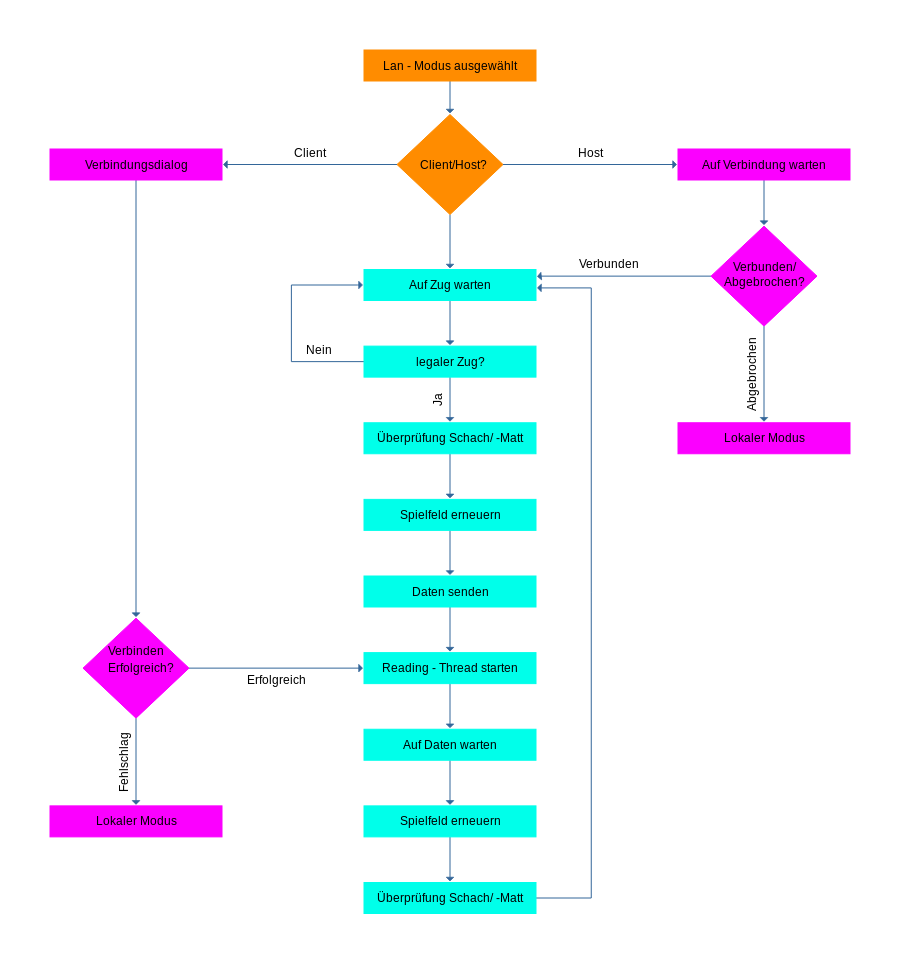
\includegraphics[width=16cm]{graphics/SpielflussLAN.png}
  \caption{Spielzyklus im LAN-Modus}
  \label{fig:lan}
\end{figure}


\subsubsection{Verbindungsvorgang des Clients}
\label{SUBSUBSEC:CONCLI}

Um mit dem Client eine Verbindung aufzubauen, muss in der Menüleiste der entsprechende Punkt angewählt. Es öffnet sich ein Dialogfenster (TODO: Verlinkung). Wird in diesem Dialogfenster der Punkt 'Join' angewählt, beginnt der Verbindungsvorgang. \\[2ex]
Ein neues Dialogfenster wird angezeigt. Der Benutzer muss hier seine IP-Adresse eingeben. 
Ist die eingegebene Adresse korrekt, so wird der Socket der LAN-Klasse mit dieser Ip-Adresse und einem fest vorgegebenen Port initialisiert. 
Ist auch dies erfolgreich, so wird das Team des Clients auf Schwarz gesetzt, die Streams zur kommunikation erstellt und es werden ein Reader Thread (TODO: Vergleich einbauen) und ein Heartbeat Thread (TODO: Vergleich einbauen) gestartet.\\[2ex]

Folgender Pseudocode zeigt den Verbingunsvorgang: \\
\lstset{language=Java}
\begin{lstlisting}

if(join ausgewaehlt){				

					wechsleSpielmodus(Lan);				
					neuerDialog();
					...							//graphisches Design des Popups
					Optional<String> ipResult = ipDialogoue.showAndWait();
					if (IP Adresse eingegeben){										
						try {
								joinAdress = eingegebene Adresse();
								SocketErstellen();
								//Streams erstellen und Teams setzen	
								StreamsErstellen()
								Verbindungsstatus(Verbunden);
								Team(Schwarz);			
								//Zugverzoegerung um einen Zug		
								Zugverzoegerung(true);
								SchachfelderKlickbar(false);
								Thread rt = new Readinthread();  		
								rt.start();
								Thread th = new HeartbeatThreadThread(Heartbeat);
								th.start();
								//Menuepunke entfernen und hinzufuegen
								menuFile.getItems().removeAll(Speichern und Laden);
								menuGame.getItems().removeAll(Spielmodi);		
								menuGame.getItems().addAll(disconnect);	
								Gui.getBoardGui().DrawGrid(Hintergrundmatrix);		
								Gui.getBoardGui().redraw();
							}

						} catch (UnknownHostException) {
							...
							spielerBenachrichtigen();
							wechsleSpielmodus(Lan);		
							
						} catch (IOException e) {
							...
							spielerBenachrichtigen();
							wechsleSpielmodus(Lan);		
						} catch (ClassNotFoundException e) {
							spielerBenachrichtigen();
							wechsleSpielmodus(Lan);		
						}
\end{lstlisting}

\subsubsection{Verbingdungsvorgang des Hosts}
\label{SUBSUBSEC:CONHOST}

Um ein Spiel zu hosten wird im Auswahldialog der entsprechende Punkt angewählt. 
Im Hintergund wird ein ein neues Spielfeld erstellt, der Spielmodus gewechselt, und es wird der 'Hosting Thread' gestartet %TODO : Verlinkung Heartbeat
Im vordergrund wird ein 'Blurry Menu' ( %TODO : Verlinkung GUI
)gezeichnet. In diesem hat der Host die Option, den Wartevorgang abzubrechen und wieder in den lokalen Modus zurückzukehren. \\
Der folgende Pseudocode zeigt, was bei dem Abbruchvorgang passiert: 
\lstset{language=java}
\begin{lstlisting}

if(Verbindungsvorgang abgebrochen){

					SchachfelderKlickbar= true; 
					//widerherstellen der Menues
					menues ruecksetzen();		
						
					try{	
						HeartbeatThreadStoppen();
						HostingThreadStoppen();}
					} catch(Exception e){
						...			 //Fehlerbehandlung
					}
						in lokalen Modus wechseln();
						DrawGrid(_BGG);
					}
				}

\end{lstlisting}

Während die Schaltfläche für den Abbruch zu sehen ist, wird im Hintergrund der Hosting Thread ausgeführt. Dieser erstellt den Serversocket, startet den Heartbeat - Thread ( %TODO : Verlinkung Heartbeat
) und wartet auf eine Verbindung. \\[2ex]
Ist der Verbindungsvorgang erfolgreich, so erzeugt der Thread den Socket der LAN - Klasse, der zum Spielen notwendig ist. ER erzeugt die Streams um die kommunikation zu ermöglichen und setzt den Verbingdungsstatus auf 'Verbunden'. \\
Anschließend muss noch die Schaltfläche zum Beenden des Wartevorganges verschwinden. Unter JavaFX kann die grafische Oberfläche allerdings nur von dem Hauptthread aus verändert werden.\\ Um dieses Problem zu umgehen wird ein Objekt der Klasse Robot erstellt. Mit diesem ist es möglich, den Mauszeiger auf die Schaltfläche zu führen und einen Klick auszulösen. 
Diser Klick wird im Hauptthrad erkannt und das Feld wird neu gezeichnet. \\
Der folgende Pseudocode zeigt die Geschehnisse im Hosting -Thread:\\
\lstset{language=java}
\begin{lstlisting}

try {
				
				HeaertbeatThread= new Thread(Heartbeat);
				TeamSetzen(Weiss);
				//warten auf eingehende Verbindung
				tempsock = VerbindungDesServersockets();
				bgg.getLan().Streams erstellen();	//erstellen der Streams
				bgg.getLan().setIsConnectet(true);
				
				//Ruecksetzen des Menues
				Point b = Position der Maus
				int xOrig, yOrig = Urspruengliche Mausposition
		      
		            try {
		                Robot r = new Robot();
		                r.mouseMove(Position des Mauszeigers);
		                r.mousecklick(linke maustaste)
		                //mauszeiger an die originale Position bewegen
		                r.mouseMove(xOrig, yOrig);
		            } catch (Exception e) {
		                ...  	//Problembehandlung
		            }
			} catch (Exception e) {
				...	//Problembehandlung
			}		
		}

\end{lstlisting}

\subsubsection{Spielfluss im LAN-Modus}

Bis auf den Verbindungsvorgang unterscheiden sich die mechaniken von Client und Host überhaupt nicht. Alle Variablen und Funktionen die notwendig sind, um den Spielfluss im LAN-Modus zu gewährleisten, sind in den Klassen 'LAN.java' und 'BoardGui.java' enthalten und werden sowohl vom Client als auch vom Host auf die Exakt gleiche Weise verwendet. Der einzige große unterschied ist, dass der Client zuerst mit dem Lesen, und der Host zuerst mit dem Schreiben von Daten beginnt. \\
Der Spielzyklus der sich ergibt wird im folgenden von Anfang an erklärt. Für ein besseres Verständnis kann das Flussdiagramm (Abb.: \ref{fig:lan}) zu Rate gezogen werden.\\
Sowohl das bewegen einer Figur, die Überprüfung, ob ein Zug erlaubt ist und die Schach/Schachmatt-Abfrage funktionieren exakt gleich wie im lokalen Spielmodus. Weiteres dazu ist im Kapitel \ref{SUBSEC:LOCAL_MODE} zu finden.\\[2ex]
Wird ein lokaler Zug erkannt, so müssen die Daten an den zweiten Mitspieler versendet werden. Um möglichst wenige Daten zu versenden und eine einfache Implementierung zu ermöglichen wird, anstatt der ganzen Backgroundgrid - Klasse nur die repräsentative Zahlenmatrix (vgl. Abb.: \ref{TABLE:REPRESENTATION-MEEPLES}) mit den aktuellen Figurenpositionen versendet. Dies geschieht über die, beim Verbinden der Spieler erstellte, Kette aus Streams. Direkt nach dem versenden wird das Feld des Spielers neu geladen und dargestellt. Um den Rundenzähler aktuell zu halten wird die Rundenzählervariable erhöht. 
Bevor das Programm in den Lesezustand geht werden die Schachfelder noch unklickbar gemacht.\\[2ex]
Um dem Spieler die Möglichkeit zu bieten, die grafische Oberfläche weiter zu benutzen und beispielsweise das Netzwerkspiel zu verlassen oder das Spiel zu beenden, wird der Lesevorgang in einen Nebenläufigen Thread ausgelagert. Dies ist notwendig, da das Programm beim Lesevorgang stehen bleiben würde und nicht weiterläuft, bis der Lesevorgang abgeschlossen ist.\\
Im folgenden wird Pseudocode angegeben, welcher den Schreibvorgang anschaulich darstellt:

\lstset{language=java}
\begin{lstlisting}

if (Bewegung legal und Lan-Modus aktiv){
				Stream.schreiben(Hintergrundmatrix);
				zeichneSpielfeld(Hintergrundmatrix);
				erhoeheRundenzaehler();
				SpielfeldKlickbar(false);
				starteReadThread();
				
}
\end{lstlisting}
Der Lesevorgang selbst wird über eine Variable getriggert, auf die ein ChangeListener aufgesetzt wird. Der Code innerhalb eines ChangeListeners wird dann ausgeführt, wenn sich die zugehörige Variable ändert. Diese Variable wird im Reader - Thread verändert, sobald das Programm bereit ist zu empfangen.
Der Code, der zum Empfangen benörtigt wird, steht zwar in der BoardGui Klasse, wird aber aufgrund der Triggerung in dem zuvor erstellten Reader - Thread ausgeführt.\\[2ex]
Beim empfangsvorgnang wird als erstes die Hintergrundmatrix neu gesetzt. Im Anschluss wird die Zuganzahl erhöht und das aktuell ziehende Team geändert.
Danach wird das Feld mit der neuen Hintergrundmatrix neu gezeichnet. Zuletzt werden noch eine Schach- und Schachmatt abfrage für beide Teams durchgeführt.\\[2ex]
Im folgenden Pseudocode wird der Empfangsvorgang anschaulich dargestellt.

\lstset{language=java}
\begin{lstlisting}

	try {

					Hintergrundmatrix=leseStream.lesen();
					Zugnummer erhoehen
					
					if (Weisses Team am Zug){
						Teamwechsel(Schwarz);
					} else if (Schwarzes Team am Zug){
						Teamwechsel(Weiss);
					}

				} catch (IOException e) {
					
					...  //Problembehandlung
				}

	BackGroundGrid.MatrixSetzen(Hintergrundmatrix);
	SpielfeldKlickbar(true);
	neuZeichnen();
	Schachmattabfage(Team Weiss);
	Schachmattabfrage(Team Schwarz);
	Schachabfrage(Team Weiss);
	Schachabfrage(Team Schwarz);
	


\end{lstlisting}


\subsubsection{Das Heartbeat - System}
\label{SUBSUBSEC:HEARTBEAT}

Ein normales Trennen der Netzwerkverbindung ist einfach zu detektieren. Schwieriger wird es, wenn die Netzwerkverbindung abbricht oder eines der beiden System aufhört zu funktionieren. In diesen Fällen ist das Programm nicht mehr in der Lage, aktiv einen Befehl zum sauberen Trennen der Netzwerkverbindung mit dem gegenüber zu versenden. Das kann dazu führen, dass ein Benutzer, der auf den Zug seines Gegners wartet, nichts von einem potentiellen Verlieren der Netzwerkverbindung oder einem Systemabsturz seines Gegenübers mitbekommet. Das führt  dazu, dass der User keine Anzeige erhält, dass sein gegenüber nicht Verbunden ist, da sich das Programm im wartezustand befinden und nur weiterläuft, sobald entsprechende Daten empfangen wurden.\\
Um dem vorzubeugen wurde ein 'Heartbeat' - System implementiert. Die idee dieses Systems ist simpel: In regelmäßigen zeitlichen Abständen, wie bei einem Herzschlag, deshalb Heartbeat, werden kleine Datenpakete über das Netzwerk zum Gegenspieler versendet. Wenn die Pakete über eine längere Zeitspanne ausbleiben, wird die Netzwerkverbindung abgebrochen.\\[3ex]
Um den Heartbeat zu realisieren kann nicht der bestehende Socket verwendet werden, da dieser damit beschäftigt ist, die Spieldaten zu senden und zu empfangen.Das bedeute, dass ein neuer Socket und ein neuer Serversocket für Client und Host erstellt werden müssen. Dieser Socket benötigt einen anderen Port, da die Computer, auf denen die Programme ausgeführt werden, sonst nicht unterscheiden könnten, welches Paket für welchen Thread gedacht ist.\\ Zusätzlich muss das ganze System auf einen zusätzlichen Thread ausgelagert werden, da es sonst die abarbeitung anderer Teile des Programmes blockiert. \\
Der Thread für den Heartbeat wird jeweils zusammen mit den Verbindungsvorgängen gestartet. Auch beim Heartbeat wird zwischen Host und Client unterschieden. 
Wenn der Thread vom Client aus gestartet wurde, wird ein neuer Socket mit der gleichen Ip-Adresse wie jener Socket, der für die Spieldaten zuständig ist, erstellt. Wenn der Thread vom Host aus gestartet wurde, wird ein Serversocket, der auf den neuen Port hört, erstellt. Dieser wartet dann auch direkt auf eingehende Verbindungen. \\
Ist ein Verbindungsvorgang erfolgreich, so erstellen beide Threads, also sowohl der vom Host, als auch der vom Client, ihre Input- und Outputstreams. Bei diesen handelt es sich um ObjectInput- und ObjectOutputStreams, die mit den lowlevel - Streams der jeweiligen Sockets verkettet werden. \\
Vor den ersten Sende- und Empfangsvorgängen wird auf jeden Socket noch ein Timer gesetzt, welcher angibt, wie lange der Thread wartet, bis er beim ausbleiben der Pakete einen Trennungsvorgang einleitet. Dieser Timer wird nach jedem empfangenen Paket zurückgesetzt.\\
Im Anschluss werden die eigentlichen Sende- und Empfangsschritte eingeleitet. Damit der Host und der Client nicht gleichzeitig mit dem Schreiben beginnen, wird eine einmalige Verzögerung beim Client eingebaut, die diesen mit dem Lesen beginnen lässt. Danach wechseln sich beide Parteien mit dem Lesen und Schreiben ab. Um das Netzwerk nicht mit 'Heartbeat - Traffic' zu fluten, wird der jeweilige Thread nach dem Senden für eine Sekunde deaktiviert.Sobald ein disconnect von Heartbeat erkannt wurde, wird mittels einer Triggervariable (also eine Variable mit Listener, ähnlich jener zum Emfpangen der Spieldaten) ein Informationsfeld gezeichnet, welches den Spieler über die verlorene Verbindung informiert. Dieses Informationsfeld ist klickbar und bringt den Spieler zurück in den Lokalen Spielmodus.\\[2ex]
Im folgenden Pseudocode werden die Anweisungen im Heartbeat-Thread veranschaulicht.

\lstset{language=java}
\begin{lstlisting}

	try {
			if(Client){
	
				Socket = new Socket(Gleiche IP,neuer Port);
				erstelleStreams(Socket);
				Socket.TimeoutNach(15 Sekunden)
			}

			else if(Host){

				Serversocket = new Serversocket(neuer Port);
				Socket = Serversocket.warteAufVerbindung();
				erstelleStreams(Socket);
				Socket.TimeoutNach(15 Sekunden)

			}
			
			while(Endlos){

					if(Erster Lesevorgang des Clients){					
					Stream.lesen();
					}

				Stream.schreiben(Testdaten);
				Thread.sleep(1000);
				Stream.lesen(Testdaten);

			}


		} catch (Exception e){
			verbindungTrennen();
			TriggervariableSetzen(); //triggert das Zeichnen der hinweisflaeche
		}
	}
\end{lstlisting}



\newpage

\subsection{AI-Mode}
\label{SUBSEC:AI-MODE}

Wie funktioniert die AI (Artificial Intelligence) des Schachspiels? \\
Für die Beantwortung dieser Frage werden folgende Kapitel behandelt:

\begin{itemize}
	\item{\nameref{SUBSUBSEC:GenAI}}
	\item{\nameref{SUBSUBSEC:OurAI}}
	\item{\nameref{SUBSUBSEC:MinMax}}
	\item{\nameref{SUBSUBSEC:AICODE}}
\end{itemize}



\subsubsection{Prinzipielle Möglichkeiten einer AI}
\label{SUBSUBSEC:GenAI}

Der Terminus ,,AI'', bzw. ,,KI'' wird sehr oft verwendet, jedoch gibt es Unterschiede zwischen den verschiedenen AIs die größer nicht sein könnten. So gibt es zum Beispiel künstliche Intelligenzen, die auf Machine-Learning-Algorithmen basieren und andere, denen ein Min-Max Prinzip zu Grunde liegt. \\
Das Min-Max Prinzip lässt sich aber nur bei Spielen mit perfekter Information anwenden, wie Schach eines ist. Ein Spiel mit perfekter Information bedeutet, dass jeder Spieler alles weiß, so haben im Schach immer beide Spieler das gesamte Spielfeld im Blick. \\[2ex]
Durch diese Art des Spiels können die theoretisch besten Züge ermittelt werden, um den besten möglichen Zug zu ziehen. Dazu muss der Algorithmus alle möglichen Spielzüge analysieren, bewerten und vergleichen, um zu einem Zug zu machen. Dies ist ein sehr hoher Rechenaufwand, dafür einfacher zu implementieren. Diese Art der AI haben wir verwendet, siehe \ref{SUBSUBSEC:OurAI}. \\[3ex]
Die andere Möglichkeit ist ein Machine-Learning-Algorithmus. Dieser versucht ein biologisches Gehirn nachzubauen, indem es ein Künstliches-Neurales-Netzwerk bildet. Diese Neuronen werden dahin gehend trainiert, dass die AI aus einem gegebenen Satz Daten und/bzw. mit Hilfe einer Lernfunktion Rückschlüsse auf mögliche zukünftige Ereignisse schließt. Mathematisch gesehen basiert diese Art der KI auf der Wahrscheinlichkeitsrechnung.  \\
Wichtig ist noch anzumerken, dass diese Art der KI selber lernen kann, damit sie besser wird. Als Beispiel nehmen wir Schach: Die KI spielt über längere Zeit gegen sich selber und muss um sich zu verbessern nicht unbedingt gegen andere Spieler, sowohl menschlich als auch maschinell antreten. \\
Maschinelles Lernen ist ein sehr umfangreiches Thema, womit hier nur noch gesagt sei, dass maschinelles Lernen in letzter Zeit einige Durchbrüche erlebt hat. Um noch ein konkretes Beispiel zu nennen: Im Dezember 2017 gewann der von Google entwickelte Algorithmus AlphaZero gegen die Chess-Engine ,,Stockfish 8''. AlphaZero basiert auf maschinellem Lernen und Stockfish 8 auf der Vorausberechnung aller möglichen Züge.\cite{SkyNet} \\[2ex]


\subsubsection{Verwendete Schach-AI-Funktion}
\label{SUBSUBSEC:OurAI}

Wie vorher schon beschrieben verwendet die Java-Chess-AI eine Abwandlung des Min-Max Algorithmus. Dieser wird ,,alphaBeta'' Algorithmus genannt. \\
Prinzipiell sucht der Algorithmus nach dem besten Spielzug. Um dies tun zu können, benötigt es einen Algorithmus, welcher alle möglichen Spielzüge bis zu einer gewissen Tiefe durchsucht und den besten Spielzug in Folge herausschreibt. \\ 
Hierfür muss geklärt werden, welcher Spieler gerade die Oberhand hat. Im entwickelten Algorithmus besteht die fundamentale ,,Board-Evaluation'' aus der materiellen Balance. Also welcher Spieler mehr und bessere Figuren hat. Anschließend werden noch  ,,Bauernformationen'', also wenn die Bauern sich gegenseitig decken und sogenannte ,,Piece Square Tables'' in die Kalkulation mit eingerechnet. Piece Square Tables geben an, wo die Figuren statistisch gesehen am besten stehen. Zum Beispiel stehen Türme lieber in der Mitte, als am Rand. Dadurch haben sie mehr Bewegungsfreiheit, was im Schachspiel eine der wichtigsten Strategien zum Sieg ist. Hierbei muss angemerkt werden, dass die Piece Square Tables von SchachmeisternInnen erstellt wurden, welche der Öffentlichkeit zugänglich gemacht worden sind.\cite{SquareTables} \\[2ex]
Das Durchsuchen der möglichen Spielzüge läuft folgendermaßen ab: Es wird zuerst festgelegt bis zu welcher Tiefe (z.B.: 5) gesucht werden soll. Anschließend wird der 1. mögliche Zug getätigt. Anschließend ruft sich die Methode selbst rekursiv auf, wobei die Tiefe erhöht und das Team gewechselt wird und tätigt wiederum den 1. möglichen Zug. Dies geschieht so lange, bis die gewünschte Tiefe (5) erreicht ist, bei welcher die ,,Board-Evaluation'' durchgeführt wird. Dieser Wert wird zwischengespeichert und der zuletzt getätigte Zug wird rückgängig gemacht. \\
Nun befindet sich der Algorithmus wieder in der Tiefe 4, in welcher der 2. mögliche Zug getätigt wird. Falls dieser Zug besser ist, als der vorherige, überschreibt dieser den zwischengespeicherten 1. Zug. Falls nicht, wird er von nun an nicht länger berücksichtigt. \\
Dies geschieht nun solange, bis alle relevanten Züge durchsucht wurden, welche nicht relevant sind wird in \ref{SUBSUBSEC:AICODE} behandelt. \\
Sobald der beste Zug ermittelt wurde, folgt die übliche Schachmatt-Abfrage und das Überschreiben des Schachfeldes mit den neuen Positionen. Anschließend ist wie in \ref{SUBSUBSEC:BLOCKSCHALTBILD} gezeigt, wieder der Spieler an der Reihe. \\[2ex]
Eines der größten Probleme des Algorithmus ist die Performance. Dazu ein simples Gedankenexperiment: Beim 1. Spielzug sind 20 mögliche Züge des weißen Spielers möglich und eben soviele beim darauffolgenden Zug des schwarzen Spielers. Daraus resultiert aus den beiden Spielzügen \(20 \cdot 20 = 400\) verschiedene Stellungen. \\
Gemittelt gibt es im Schach 28 mögliche Züge pro Spielzug. Nach 5 Zügen ergeben sich daraus schon 3.200.000 mögliche Stellungen, nach 6 wären es 64.000.000. Um zu einer Entscheidung zu kommen, muss der Computer alle diese Züge analysieren und bewerten. Dies benötigt Rechenleistung, weshalb ein solcher Schachalgorithmus sehr abhängig von der verwendeten Hardware ist. \\
Im weiteren Sinne ist dies der Grund, warum solche künstlichen Intelligenzen gegen Künstliche-Neuronale-Netzwerke verlieren (siehe \ref{SUBSUBSEC:GenAI}). Die Min-Max Algorithmen können nicht ausreichend optimiert werden bzw. moderne Hardware besitzt einfach nicht genügend Rechenleistung, um in diesem Wettlauf mithalten zu können. \\

\subsubsection{Der MinMax-Algorithmus:}
\label{SUBSUBSEC:MinMax}

In den Kapiteln \ref{SUBSUBSEC:GenAI} und \ref{SUBSUBSEC:OurAI} wurde erwähnt, dass die JavaChess AI nach dem Min-Max Prinzip funktioniert, nur was ist dieses Prinzip?

\begin{figure}[H]
  \centering
   	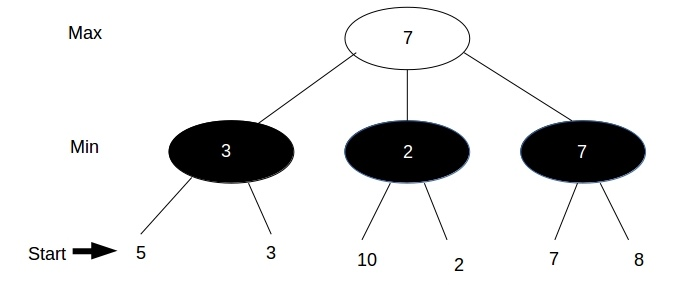
\includegraphics[width=16cm]{graphics/MinMax.jpg}
  \caption{Min-Max}
  \label{FIG:MINMAX}
\end{figure}


MinMax ist nichts anderes, als das Erhalten des bestmöglichen Ergebnisses für einen Spieler, wenn die Züge des Gegenspielers mit eingerechnet werden. In diesem Beispiel haben wir zwei Teams, Weiß und Schwarz. Diese sind durch die weißen Blasen erkenntlich. Weiters gilt für ein kompetitives Spiel wie Schach, dass das weiße Team immer ihr bestes Ergebnis herausholen möchte und das Schwarze auch ihres. Die Zahlen repräsentieren die Günstigkeit der Stellung für das weiße Team, wobei 10 die bestmögliche Stellung ist und 1 die schlechteste. Für das schwarze Team ist dies umgekehrt, für sie ist 10 das schlechteste Ergebnis und 1 das Beste. \\
Somit wird das schwarze Team immer das kleinere Ergebnis nehmen, quasi das MINIMUM herausholen (=Min) und die Weißen immer das höchstmögliche, also das MAXIMUM (=Max). Daher auch der Name, MinMax. \\
Zurück zum Beispiel: Schwarz kann einmal wählen zwischen den Zahlen 5 \& 3, zwischen 10 \& 2 und zwischen 7 \& 8. Da die Schwarzen immer die niedrigere Zahl nehmen, kann die niedrigere Zahl in den schwarzen Bubble geschrieben werden (3, 2 \& 7). \\
Somit muss sich der weiße Spieler nur noch zwischen 3 Zahlen entscheiden, bei denen er die höchste nimmt, also 7. Dies ist das bestmögliche Ergebnis für das weiße Team.

\subsubsection{Code}
\label{SUBSUBSEC:AICODE}

Die theoretischen Grundlagen zum Verständnis des Algorithmus sollten nun geklärt sein.\\
Die KI besteht aus zwei Klassen, AI und AILogic. AI wird als neuer Thread ausgeführt. \\
Der nachfolgende Code zur AI erfolgt als Pseudo-Code Dokumentation.


Klasse AI:

\lstset{language=Java}
\begin{lstlisting}
	public class AI extends Thread{
		public void run(){
			AIL = initialisiere AILogic()
			AIL.alphaBeta()
			//Besten Zug bekommen
			Move = AIL.getMove()
			
			Hintergrundmatrix mit Move veraendern.
		}
	}	
\end{lstlisting}

Klasse AI-Logic:
\lstset{language=Java}
\begin{lstlisting}
	public class AILogic{
	
		private MaximaleTiefe
		//wird benoetigt um die maximale Tiefe festzulegen und um den Logarithmus zu verbessern
		public float alphaBeta(tiefe, Hintergrundmatrix, Team){
			MaximaleTiefe = tiefe
			alpha = 10000
			beta = -10000
			for(i<tiefe){
				//Fuer den AlphaBeta algorithmus
				beta = alphaBetaHelper(starte bei Tiefe 0, BackgroundMatrix, alpha,beta)
			}
			
		}	
	
		//der AlphaBeta Algorithmus - zur Zugevaluation 
		public float alphaBetaHelper(tiefe, Hintergrundmatrix, Team, alpha, beta){
			Sum = boardEvaluation
			
			if(Sum bedeutet das feindlicher Koenig geschlagen wird){
				return 20000
			}
			
			if(tiefe >= MaximaleTiefe){
				return Sum
			}
			
			for(X und Y Positionen des Spielfeldes){
				if(Spielfigur an Position){
					Zuege = AlleMoeglichenZuegeDerSpielfigur
					for(alle Moeglichen Zuege der Figur){
						A = Zug						
						Den Zug auf das Spielfeld uebertragen
						
						Sum1 = -alphaBetaHelper(tiefe+1, BackgroundGrid, Teamwechsel, -alpha, -beta)
						
						Den Zug rueckgaengig machen		
						
						if(Sum1 >= beta){
							beta = Sum1	
							if(Sum1 >= alpha){
								return alpha
							}			
							if(tiefe == 0){
								ZuListeGuterZuegeHinzufuegen(A)						
							}
						}	
						
					}
				}
				
			}
		return beta			
		}
		
		public float boardEvaluation(Backgroundgrid, Team){
			//Fuer die Material Balance
			
			for(X und Y Positionen des Spielfeldes){
				if(Bauer weisses Team){
					100 Punkte zum weissen Team dazu zaehlen
					Punkte entsprechend der Bauerntabelle hinzuzaehlen
					Punkte nach Bauerntabelle hinzuzaehlen
				} else if(Turm weisses Team){
					500 Punkte zum weissen Team dazu zaehlen
					Punkte entsprechend der Turmtabelle hinzuzaehlen
				} else if(Springer weisses Team){
					325 Punkte zum weissen Team dazu zaehlen
					Punkte entsprechend der Springertabelle hinzuzaehlen
				} else if(Lauefer weisses Team){
					300 Punkte zum weissen Team dazu zaehlen
					Punkte entsprechend der Lauefertabelle hinzuzaehlen
				} else if(Dame weisses Team){
					900 Punkte zum weissen Team dazu zaehlen
					Punkte entsprechend der Damentabelle hinzuzaehlen
				} else if(Koenig weisses Team){
					10000 Punkte zum weissen Team dazu zaehlen
					Punkte entsprechend der Koenigtabelle hinzuzaehlen
				}
				
				if(Bauer schwarzes Team){
					100 Punkte zum schwarzen Team dazu zaehlen
					Punkte entsprechend der Bauerntabelle hinzuzaehlen
					Punkte nach Bauerntabelle hinzuzaehlen
				} else if(Turm schwarzes Team){
					500 Punkte zum schwarzen Team dazu zaehlen
					Punkte entsprechend der Turmtabelle hinzuzaehlen
				} else if(Springer schwarzes Team){
					325 Punkte zum schwarzen Team dazu zaehlen
					Punkte entsprechend der Springertabelle hinzuzaehlen
				} else if(Lauefer schwarzes Team){
					300 Punkte zum schwarzen Team dazu zaehlen
					Punkte entsprechend der Lauefertabelle hinzuzaehlen
				} else if(Dame schwarzes Team){
					900 Punkte zum schwarzen Team dazu zaehlen
					Punkte entsprechend der Damentabelle hinzuzaehlen
				} else if(Koenig schwarzes Team){
					10000 Punkte zum schwarzen Team dazu zaehlen
					Punkte entsprechend der Koenigtabelle hinzuzaehlen
				}
			}
		}
		
		...Tabellen fuer Bauern, Lauefer,...		
		
	}	
\end{lstlisting}
%\lstset{language=German}

%=================================================================================
\clearpage\vfill\newpage{}
%=================================================================================
\section{ChessPI}
\label{SEC:chesspi}

ChessPI ist die Implementierung von JavaChess auf dem Raspberry PI. \\
Wir haben uns zur Aufgabe gestellt, dass das Schachprogramm auch auf einem Mikro-Computer, wie dem RaspberryPI 3b, läuft. An dem RaspberryPI wird ein Touchscreen angeschlossen, mit welchem der User interagieren kann. Weiters soll für den RaspberryPI mit angeschlossenen Touchscreen ein Gehäuse designt und eine Akkusteuerung entworfen werden. 
Die Probleme die dabei auftreten können sind unzählig, die Hauptprobleme können aber determiniert werden:
\begin{itemize}
	\item{Der RaspberryPI besitzt zu wenig Rechenleistung}
	\item{Die verfügbaren Java Versionen beinhalten nicht die von uns verwendeten Packages}
	\item{Das Spiel ist nicht über einen Touchscreen spielbar}
\end{itemize}

\subsection{RaspberryPI}

Der Raspberry PI ist ein vollwertiger Computer, welcher mit einem Linux/GNU OS läuft. Am häufigsten wird die Distribution Raspbian verwendet. \\
Die von uns verwendete Version ist der Raspberry PI 3 model B. Dieser verfügt über eine Quad Core 1.2 GHz Broadcom BCM2837 CPU, 1 GB an RAM.\cite{RaspiSpecs} Dies ist eine deutliche Steigerung gegenüber den vorherigen Modellen, womit das Problem notwendige Leistung zumindest leicht gelöst wird. \\

\subsection{Touchscreen}

Als Touchscreen wird das Ofizielle 7" Touchscreen Display verwendet. Dies hat eine Auflösung von 800x480 Pixel.\cite{RaspiScreen} \\
Zusätzlich zum Display gibt es auch eine Adapterplatine, mit der der Touchscreen versorgt wird. \\
Halterungen für die Adapterplatine und den Raspberry PI gibt es auf der Rückseite des Touchscreens.

\subsection{Implementierung von JavaChess}

Alle benötigten Schritte beziehen sich lediglich auf die Software Implementation, nicht auf die Hardware Implementation (Powerbank, Gehäuse). \\[1ex]

\textbf{Vorbereitung:} \\[2ex]
Es wird ein RaspberryPI 3, eine Mikro SD-Karte mit Raspbian, eine Stromversorgung bzw. eine Powerbank mit einem maximalen Strom von 2.5 A, der 7" Touchscreen, die Adapterplatine, eine Internetverbindung idealerweise über ein LAN-Kabel und eine USB-Tastatur benötigt. \\

\begin{enumerate}
	\item{Die SD Karte mit Raspbian wird in den Raspberry PI gegeben}
	\item{Die Adapterplatine und der Raspberry PI wird auf den Touchscreen geschraubt}
	\item{Die Stromversorgung für den Display (VCC \& GND Pin- rotes und blaues Kabel) wird sichergestellt. Das Flachbandkabel / Datenkabel wird zwischen Raspberry PI und Adapterplatine angebracht.}
	\item{Der Raspberry Pi wird an die Stromversorgung angeschlossen, dadurch sollte dieser nun booten und den Display automatisch erkennen.}
	\item{Sobald Raspbian gebootet hat, wird das LAN-Kabel angeschlossen.}
	\item{Nun sollten folgende Befehle in der BASH ausgeführt werden:}
	\begin{enumerate}
		\item{sudo apt-get update}
		\item{sudo apt-get upgrade}
		\item{sudo apt-get install oracle-java8-jdk}
		\item{reboot}
	\end{enumerate}
	\item{Nun wurde Java installiert. Es muss noch JavaFX ,,dazuinstalliert'' werden, da dies nicht in der Java-Embedded-JDK Serie enthalten ist.}
	\item{Es muss OpenJFX gedownloaded werden. URL: https://chriswhocodes.com/}
	\item{Hier die Version für den Raspberry PI downloaden (ARMv6)}
	\item{Die gedownloadete OpenJFX Zip muss im Installationsverzeichnis ovn Java-JDK8 ,,unzipped'' werden.}
	\item{In Commandline wird nun folgender Befehl ausgeführt: unzip openjfx-sdk-overlay-linux-arm6hf.zip -d /<installations-verzeichnis-von-Java (z.B.: /home/pi/jdk1.8.0\_92)>}
	\item{Nun wird das aktuelle Schachspiel gedownloaded (die Jar), URL: https://github.com/alexl4123/diplomarbeit/releases}
	\item{Das Schachspiel wird in das Verzeichnis der Wahl abgelegt.}
	\item{Nun kann das Schachspiel gestartet werden, dazu muss der Touchscreen aber noch konfiguriert werden, da sonst ein ,,interessanter'' Offset geschieht.}
	\item{Dazu muss zuerst der Touchscreen identifiziert werden: cat /sys/class/input/event1/uevent}
	\item{Bei dem Versuchs-Raspberry PI war dieses Input Device: 0/0/0/0}
	\item{Um das Schachspiel bequem zu öffnen wird empfohlen ein BASH-Skript zu erstellen:}
	\item{\# /bin/bash \\
	java -Dmonocle.input.0/0/0/0.minX=0 -Dmonocle.input.0/0/0/0.minY=0 -Dmonocle.input.0/0/0/0.maxX=800 -Dmonocle.input.0/0/0/0.maxY=500 -jar chess.jar}
	\item{Nun das Skript öffnen: sudo ./<skript>}
	\item{Das Schachspiel sollte sich nun öffnen.}
\end{enumerate}
	

%TODO

%=================================================================================
\clearpage\vfill\newpage{}
%=================================================================================
\section{Akkusteuerung}
\label{SEC:AKKUSTEUR}

Ziel ist es eine Akkusteuerung zu entwerfen. Diese soll es ermöglichen, den ChessPI auch unterwegs verwenden zu können. \\
Die mobile Spieldauer soll größer einer Stunde sein. \\[1ex]
Für eine Akkusteuerung gibt es prinzipiell mehrere Möglichkeiten, angefangen bei der Powerbank, über bestimmte ICs bis hin zu einer selbst entwickelten Akkusteuerung. \\

\subsection{Kenngrößen des benötigten Akkumulators}
\label{SUBSEC:AKKU-NEEDS}

Um einen Akku auswählen zu können, muss zuerst einmal definiert werden, was gebraucht wird.\\
\begin{itemize}
	\item{Minimale Betriebsdauer $t_{min}= 1h$}
	\item{Stromaufnahme RaspberryPI-Max: $I=2.5A_{\cite{RaspiPower}}$ - zu beachten ist hierbei, dass die Stromaufnahme bei angeschlossenem Bildschirm ca. 2 Ampere beträgt, falls noch weitere Peripheriegeräte angeschlossen werden, erhöht sich die Stromaufnahme entsprechend.}
	\item{Versorgungsspannung RaspberryPI: $U_V = 5V$}
\end{itemize}

\subsection{Wählen des Akkumulators}
\label{SUBSEC:CHOOSE-AKKU}

Akkumulatoren Typen gibt es viele, für den Einsatz als RaspberryPI Versorgung schieden alle aus bis auf folgende Akkumulatorentypen: Lithium-Ionen (Li-Ion), Nickel-Cadmium (NiCd),  Lithium-Polymer (LiPo) und Lithium-Eisenphosphat ($LiFePO_4$). Jeder dieser Akkutypen bietet verschiedene Vorteile, so bietet LiPo relativ hohe Entladeströme und Li-Ion eine ziemlich hohe Energiedichte $_{\cite{wiki:akku}}$. \\
Für den Einsatz als Versorgung für den RaspberryPI sollte ein Akku möglichst an die 5V Versorgungsspannung heran kommen. Dies in Betracht gezogen, scheiden NiCd (1.2V) und $LiFePO_4$ (3.3V) ebenfalls aus. \\
So bleiben entweder der LiPo (3.7V) oder der Li-Ion (ca. 3.6V) Akkumulator übrig. Von beiden wurden gleichwertige Akkus verglichen, aufgrund der niederen Kosten eines $Li-Ion_{\cite{akku-liion}}$ Akkumulators gegenüber eines $LiPo_{\cite{akku-lipo}}$ Akkumulators, ist die Entscheidung für den Li-Ion Akku gefallen.

\subsection{Der Li-Ion Akku}
\label{SUBSEC:LIION}

Der Lithium-Ionen Akkumulator wird durch das Konstantspannungs-Ladeverfahren geladen. Hierbei wird eine Spannungsquelle mit konstanter Spannung an den Akku angeschlossen. Eingestellt wird die Spannung auf die Standardladespannung des Akkus. Bei 3.7V nominaler Spannung ist die Ladespannung typ. 4.2 Volt. \\
Die minimal benötigte Kapazität berechnet sich wie folgt, wenn eine Stromaufnahmen von 2.5 Ampere angenommen wird.:
\[Q_{min} = t*I = 1h * 2.5A = 2.5 Ah = 2500 mAh\]
Bei der Verkäuferseite Reichelt wurde ein Akku mit diesen Vorgaben gefunden: \cite{akku-liion}\\
Dieser Akku hat eine maximale Kapazität von 2600 mAh, einen maximalen Entladestrom von 2.5 A und eine Ladespannung von 4.2V. \\[1ex]
Das Datenblatt zu allen technischen Eigenschaften befindet sich auf der Seite von Reichelt (\cite{akku-liion}).

\subsection{Idee der 1. Akkusteuerungsschaltung}
\label{SUBSEC:AKKUSTEUR1}

Die ursprüngliche Idee war es, die Akkus über eine Micro-USB Buchse zu laden und damit den Raspberry PI zu betreiben. Da USB eine Spannung von 5V aufweist, muss diese zum Laden der Akkus auf 4.2 V reduziert werden. Für den Betrieb des Raspberry PIs muss diese Spannung wieder auf 5V erhöht werden. \\
Geladen werden die Akkus parallel und entladen seriell, so muss eine Schaltung entwickelt werden die eine Umschaltung von seriell auf parallel und umgekehrt ermöglicht. \\
Weiteres muss die Schaltung für den sicheren Betrieb der Akkus sorgen, so muss diese bei Unter- oder Überspannung abschalten und falls ein Kurzschluss auftritt Schlimmeres verhindern. \\
Eine Akkuladestandanzeige wird mittels zwei LEDs realisiert, die eine schaltet bei 1/3 VCC und die andere bei 2/3 VCC. 

\subsubsection{Laden der Akkus}
\label{SUBSUBSEC:AKKULOAD1}

Durch die Eingangsschaltung der Akkus wird die Versorgungsspannung auf unter 4.2 Volt gesenkt. Dies geschieht durch zwei in Serie liegende Dioden, eine SI-Diode mit einer Durchschaltspannung von ca. 0.7V und eine Ge-Diode mit einer Durchschaltspannung von ca. 0.2V. \\
Der Ladestrom darf maximal 2.5A betragen, sollte aber geringer sein, um den Akku nicht zu beschädigen. Als Begrenzung kommt ein Leistungsvorwiderstand zum Einsatz. Dieser hat 4$\Omega$ und begrenzt den Strom auf 1.25 Ampere. \\
Da die Akkus parallel geladen werden, muss dies für jeden Akku einzeln aufgebaut werden. \\
In Punkt \ref{SUBSUBSEC:CIRCUIT-1} befindet sich die Schaltung des 1. Versuchs. Folgende Bauteile dieser Schaltung werden ausschließlich für das Laden verwendet:\\
 $D_1,R_{sen1},R_{sen2},D_{s8},D_{S2},S_{I1},S_{I2}, Akku1, Akku2$ \\


\subsubsection{Entladen der Akkus}
\label{SUBSUBSEC:AKKUENTLOAD1}

Das Entladen der Akkus erfolgt durch die Seriellschaltung der Akkus (siehe \nameref{SUBSUBSEC:SERPAR}). Seriell geschalten addiert sich die Spannung der beiden Akkus auf 7.4 Volt. Diese Spannung wird mittels StepDown Converter (LM2596) auf 5 Volt herunter geregelt.  Dies kann als Versorgung für den Raspberry PI verwendet werden. \\
Die Beschaltung erfolgt gemäß des Datenblattes (Siehe \cite{LM2596}) . Die Berechnung der beiden Widerstände erfolgt ebenfalls gemäß Datenblatt.
\[R_2 = R_1 \cdot \left(\frac{V_{out}}{V_{ref}} - 1 \right)\]
\[V_{ref} = 1.25 V - R_1 = 1 k\Omega - V_{out} = 5V\]
\[R_2 = 1000*(4-1) = 3 k\Omega\]

Zum ein und ausschalten des Raspberry PIs wird noch ein Schalter verbaut. \\
In Punkt \ref{SUBSUBSEC:CIRCUIT-1} befindet sich die Schaltung des 1. Versuchs. Folgende Bauteile dieser Schaltung werden ausschließlich für das Entladen verwendet:\\ $LM2596,C_1,D_{s1},L_1,R_1,R_2,C_2,Schalter,Akku1, Akku2$ \\

\subsubsection{Seriell-Parallel Schaltung}
\label{SUBSUBSEC:SERPAR}

Die Seriell-Parallel Umschaltung ermöglicht das wechseln zwischen dem parallelen Laden und dem seriellen Entladen. Es wird erkannt, ob eine Versorgung angeschlossen ist. Wenn diese angeschlossen ist, schalten die Transistoren so, dass der ohmsche Widerstand zwischen den beiden Akkus zu groß ist, um einen Einfluss auf die Schaltung zu haben.\\
Weiteres wird das Potential des negativen Anschlusses des 2. Akkus auf Ground gesetzt um das Laden zu ermöglichen. Die Versorgung wird direkt vor den Schalter des Ausganges gehängt, womit der Akku überbrückt wird, damit der Akku sich nicht gleichzeitig entladen und laden muss. \\[2ex] 
Sobald das Micro USB Kabel aus gesteckt wurde, wird das Potential von VCC (Micro USB nicht vorhanden - also undefiniert) auf GND gehängt. Die Verbindung zwischen dem Pluspol des Akku1 und dem Minuspol des 2.Akkus wird wieder hergestellt. Dabei wird die Verbindung zwischen dem Minuspol des 2.Akkus und GND aufgehoben, um einen Kurzschluss zu verhindern.  \\
Die Verbindung zwischen dem 2.Akku und dem LM2596 wird aufgetrennt, um ein Entladen des Akkus zu verhindern. \\
In Punkt \ref{SUBSUBSEC:CIRCUIT-1} befindet sich die Schaltung des 1. Versuchs. Folgende Bauteile dieser Schaltung werden ausschließlich für das Entladen verwendet:\\ $T_1,R_{T1},T_3,R_{T3},T_6,R_{T6},T_{m3},T_{m4}, Akku1, Akku2$ \\

\subsubsection{Sicherheit}
\label{SUBSUBSEC:Security}

Unter Sicherheit werden alle Sicherheitsmaßnahmen verstanden, die eine Fehlfunktion des Akkus verhindern. \\
Dafür gibt es einen Spannungsteiler, welcher alle kritischen Spannungen für Komperatoren zu Verfügung stellt. \\
Die Spannungen sind: 
\begin{itemize}
	\item{Minimale Abschaltspannung: $U_{ref4} = 3 V$}
	\item{Akku zu 33\% geladen:$ U_{ref3}=3.3V$}
	\item{Akku zu 66\% geladen: $U_{ref2} = 3.7V$}
	\item{Maximale Ladespannung erreicht: $U_{ref1} = 4.1V$}
\end{itemize}

Wird die minimale Spannung unterschritten, wird die Verbindung zwischen Ausgang und den Akkus gekappt. \\
Wird die maximale Ladespannung erreicht, wird die Verbindung zwischen VCC und den Akkus getrennt. Diese beiden Schutzmechanismen werden für jeden Akku verbaut.\\
In der Schaltung sind drei Vieramperesicherungen verbaut, diese sorgen für die nötige Kurzschlusssicherheit.  \\
Die Spannungen $ U_{ref3}=3.3V und U_{ref2} = 3.7V$ geben den Ladestand des 1.Akkus an. Zwei Komperatoren vergleichen fortlaufend die Referenzspannungen mit der Akkuspannung und geben über zwei LEDs den Akkustand wieder. Da beide Akkus immer den gleichen Ladestand haben sollten, braucht man keine zusätzliche Schaltung für den 2. Akku.
In Punkt \ref{SUBSUBSEC:CIRCUIT-1} befindet sich die Schaltung des 1. Versuchs. Folgende Bauteile dieser Schaltung werden ausschließlich für das Entladen verwendet:\\ $OPV_1, OPV_2,T_2,T_4, T_5,LED_1,LED_2,R_{LED1},R_{LED2},R_{T2}, R_{T4},T_{T5}$ 
\newpage
\subsubsection{Schaltung}
\label{SUBSUBSEC:CIRCUIT-1}
\begin{figure}[H]
  \centering
		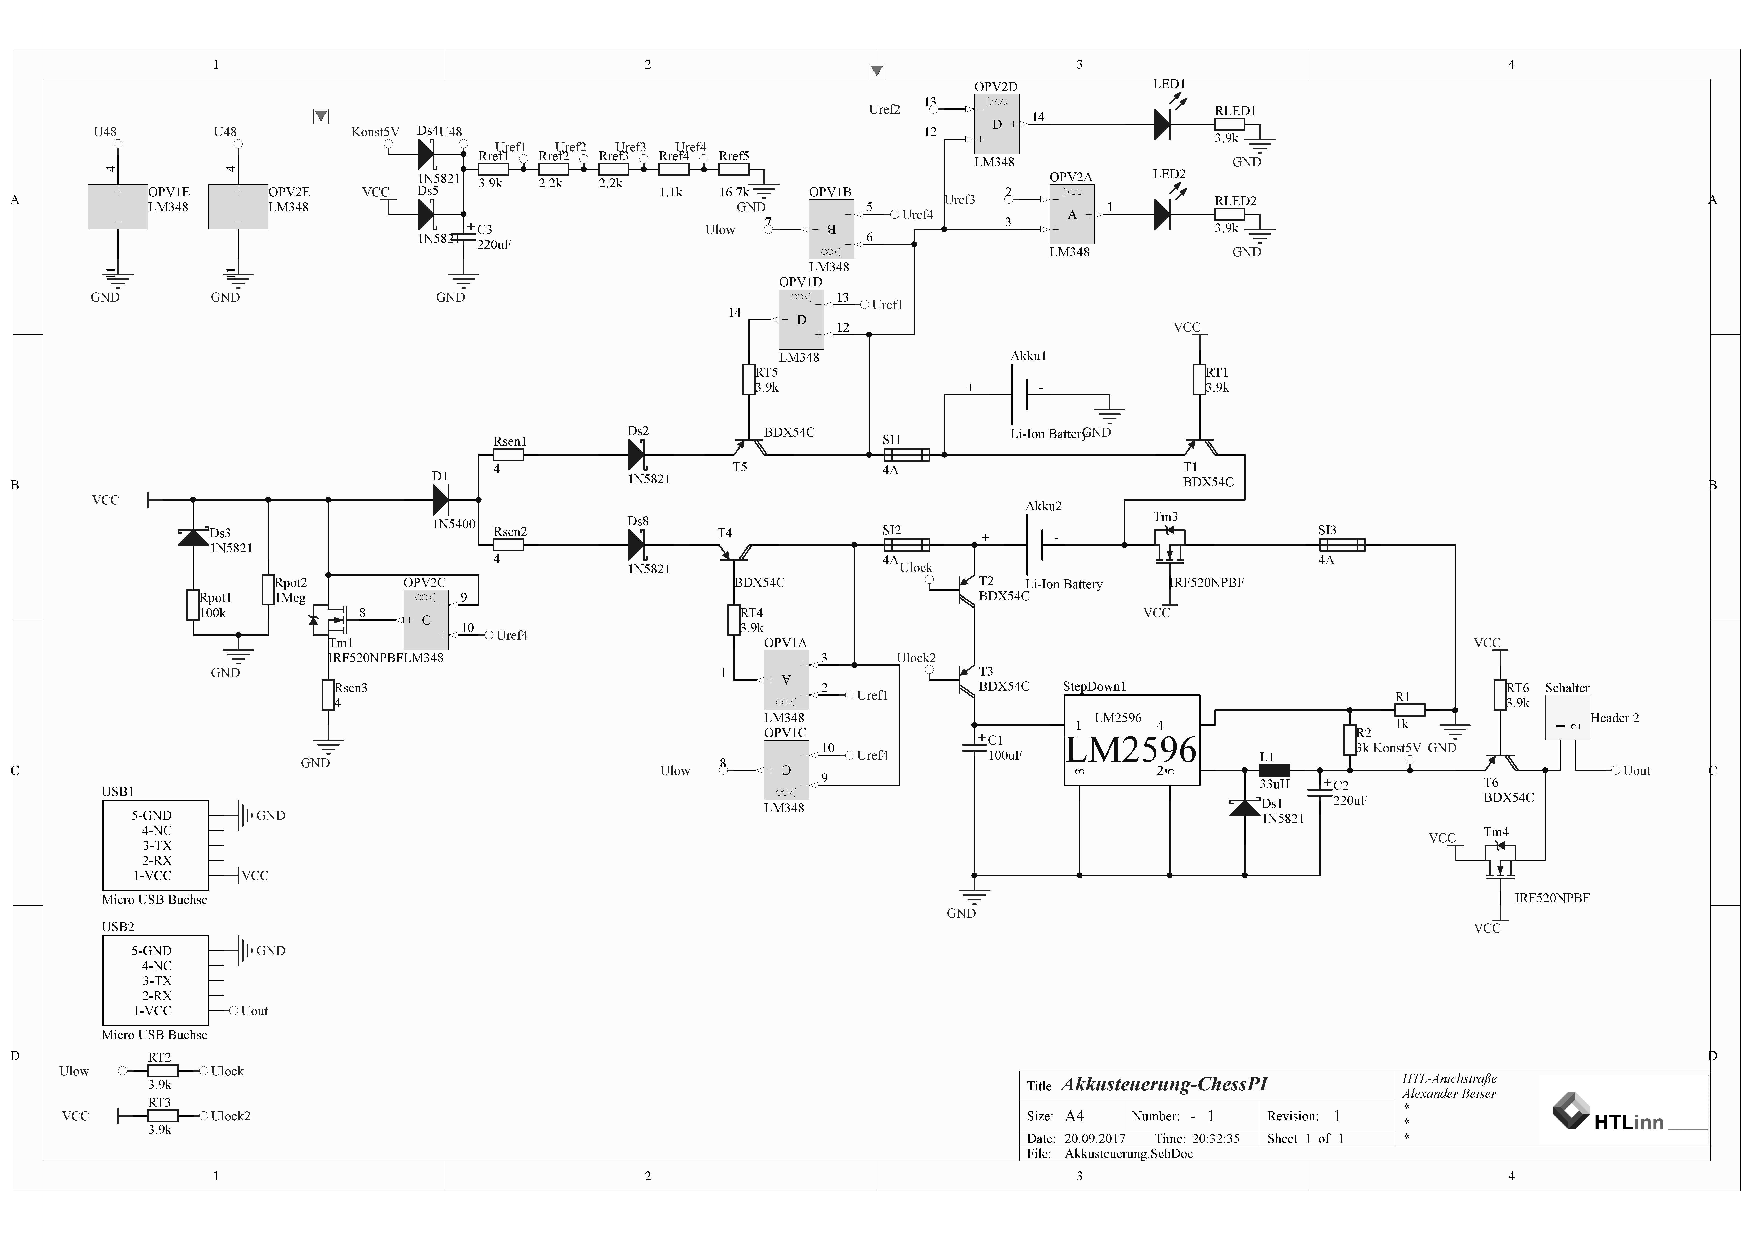
\includegraphics[scale=0.7, angle=90]{graphics/20170920-Shematic.pdf}
		\caption{Die 1.Schaltung}
		\label{fig:circuit1}
\end{figure}

\newpage
\subsubsection{Messung}
\label{SUBSUBSEC:MEASUREMENT1}

Alle Messungen wurden auf mehreren Steckbrettern aufgebaut. \\
Die Messung wurde in mehrere Phasen gegliedert:
\begin{enumerate}
	\item{Messung der Ausgangsschaltung}
	\item{Messung der Eingangsschaltung}
	\item{Umschalten der zwischen den Schaltungen}
	\item{Gesamtschaltungsmessung}
\end{enumerate}

\textbf{Messung der Ausgangsschaltung:}  Es wurden lediglich die in \ref{SUBSUBSEC:AKKUENTLOAD1} erwähnten Bauteile verwendet. Damit die Akkus nicht gefährdet werden, wird die Messung mit einem Labornetzteil durchgeführt. \\
Dieses wird auf 8.4V (max Akkuspannung) gestellt, anschließend wird der Ausgang gemessen. \\
Die Ausgangsspannung beträgt wie gewünscht 5V.
Der maximale Ausgangsstrom beträgt mit $T_6$ lediglich 2 Ampere, ansonsten 3.2 Ampere. $T_6$ wird hierbei voll ausgesteuert. 2 Ampere reichen für den RaspberryPI ohne Peripherie aber mit Display aus. \\
Anschließend wird die Messung mit den Akkus wiederholt, wobei sich das Ergebnis nicht wesentlich ändert.\\[2ex]

\textbf{Messung der Eingangsschaltung:} Es wurden lediglich die in \ref{SUBSUBSEC:AKKULOAD1} erwähnten Bauteile verwendet. Die Akkus werden sofort eingebaut. Als VCC wird ein Labornetzteil verwendet, welches auf VCC=5V eingestellt wird. \\
Die Messung der Spannungspunkte ergibt das jeweils gewünschte Ergebnis. \\
Der Ladestrom ist aber viel zu niedrig, 2 mA. Zu Testzwecken werden die Sicherheitstransistoren $T_4 und T_5$ ausgebaut. Ohne diese beiden Transistoren kommt man auf einen maximalen Eingangsstrom von ca. 25 mA, was ebenfalls zu niedrig ist. \\
Es werden noch mehrere Versuche unternommen die Schaltung zu retten, was aber nicht gelingt. Somit wird eine komplett neue Eingangsstufe entworfen, siehe \nameref{SUBSEC:AKKUSTEUR2}(\ref{SUBSEC:AKKUSTEUR2}).

\newpage
\subsection{Idee der 2. Akkusteuerungsschaltung}
\label{SUBSEC:AKKUSTEUR2}

Die 2.Akkusteuerungsschaltung unterscheidet sich primär von der 1. in der Eingangsschaltung bzw. der Akkuladeschaltung. Diesmal sind die Akkus ständig in Serie geschalten. Die Sicherheitsvorkehrungen wurden reduziert, sind aber immer noch ausreichend.

\subsubsection{Laden der Akkus}
\label{SUBSUBSEC:AKKULOAD2}

Das Micro-USB Kabel hat wiederum 5V Versorgungsspannung. Die beiden Akkus sind in Serie geschaltet, womit die Ladespannung 8.2V (2*4.1V) betragen muss. Diese Spannung wird durch einen StepUp Converter vom Typ LT1370 erreicht. Dieser ist ein verstellbarer StepUpDownConverter. \\
Die Beschaltung des ICs und die Formel, zur Berechnung der Widerstände, wird wiederum aus dem Datenblatt entnommen (\cite{LT1370}). \\
\[V_{out}=8.2V;V_{ref}=1.245V;R_{SU2}=10k\Omega\]
\[V_{out}=V_{ref} \cdot \left( 1 + \frac{R_{SU1}}{R_{SU2}} \right)\]
\[R_{SU1} = R_{SU2} \cdot \left( \frac{V_{out}}{V_{ref}} - 1 \right) = 55.8 k\Omega \rightarrow E-12 \rightarrow R_{SU1} = 56 k \Omega\]

\vspace{1cm}
Dieses Widerstandsverhältnis transformiert die Spannung von 5V auf 8.2V, womit die in Serie geschalteten Akkus geladen werden können.  \\
In Punkt \ref{SUBSUBSEC:CIRCUIT-2} befindet sich die Schaltung des 2. Versuchs. Folgende Bauteile dieser Schaltung werden ausschließlich für das Laden verwendet:\\ $LT1370,C_{SU1},C_{SU2},C_{SU3}, L_{SU1},R_{SU1},R_{SU2},R_{SU3},D_{SU1}$ 

\subsubsection{Entladen der Akkus}
\label{SUBSUBSEC:AKKUENTLOAD2}

Die Entladeschaltung der 2.Schaltung entspricht exakt der Entladeschaltung des 1.Versuches (siehe: \nameref{SUBSUBSEC:AKKUENTLOAD1} (\ref{SUBSUBSEC:AKKUENTLOAD1})).\\
In Punkt \ref{SUBSUBSEC:CIRCUIT-2} befindet sich die Schaltung des 2. Versuchs. Folgende Bauteile dieser Schaltung werden ausschließlich für das Laden verwendet:\\ $LM2596,D_{S1},L_{SD1},C_{SD2},R_{SD1},R_{SD2}$. 
\newpage

\subsubsection{Sicherheit}
\label{SUBSUBSEC:Security}

Als Sicherheit wird wiederum ein Über- und Unterladeschutz verwendet. So gibt es eine automatische Abschaltung, wenn der Akku vollgeladen oder entladen ist. Die Überwachung greift für jeden Akku einzeln, dies geschieht wieder über Komperatoren, aber nur einen Transistor. Dieser sperrt, wenn der Schutz greift und ist geöffnet, wenn der Akku geladen oder verwendet werden darf. \\
Um den Schutz beider Akkus zu ermöglichen, ist in der Serienschaltung eine Subtrahiererschaltung eingebaut. Die Differenz dieser Schaltung ergibt den momentanen Ladezustand des 2.Akkus.\\
Die Referenzspannungen der Komperatoren ergeben sich aus einem Spannungsteiler und ergeben:
\begin{itemize}
	\item{$V_{41} = 4.1V$}
	\item{$V_3 = 3V$}
\end{itemize}
\subsubsection{Messung}
\label{SUBSUBSEC:MEASUREMENT2}

Die Ausgangsschaltung wurde schon in \ref{SUBSUBSEC:MEASUREMENT1} gemessen und kann somit ausgelassen werden.  \\
Das Hauptaugenmerk liegt auf der Eingangsstufe, welche die 1.Schaltung nutzlos gemacht hat. \\

\textbf{Eingangsschaltung: }Die Messung der Eingangsschaltung erfolgt auf einem Steckbrett. VCC wird mittels einem Labornetzteil bereitgestellt. Dieses wird auf 5V eingestellt. \\
Die Spannungslevel stimmen bei allen Messpunkten. Der Eingangsstrom ist aber wiederum viel zu niedrig (10 mA mit $T_1$, ohne 50 mA). \\
\textbf{Sicherheit:} Es wird überprüft, ob die Sicherheitsabschaltung funktioniert, dazu wird anstatt den Akkus ein Labornetzteil gehängt, welches einmal auf 8V Vout und einmal auf 2.5V Vout eingestellt wird. Durch diese Einstellung wird der Transistor $T_1$ hochohmig. \\
Die Schaltung kann somit theoretisch, als sichere Ladeschaltung verwendet werde. Der Haken dabei ist, dass das Laden eines Akkus eine Woche dauert. Da das Entwickeln einer neuerlichen Schaltung aufgrund zeitlicher Beschränkungen nicht mehr möglich ist, wird eine Einigung mit Prof. Signitzer getroffen. \\
In dieser wird als Akkumulator+Schaltung eine Powerbank verwendet, für technische Daten siehe \ref{SUBSEC:POWERBANK}.

\subsubsection{Schaltung}
\label{SUBSUBSEC:CIRCUIT-2}
\begin{figure}[H]
  \centering
	%	\includegraphics[scale=0.7, angle=90]{graphics/20171104-Shematics.pdf}
		\caption{Die 2.Schaltung}
		\label{fig:circuit2}
\end{figure}

\newpage
\subsection{Verwendete Lösung}
\label{SUBSEC:POWERBANK}

Um einen ChessPI Prototypen rechtzeitig fertigzustellen, wird auf eine eigen entwickelte Schaltung innerhalb des ChessPI verzichtet. Stattdessen soll eine Powerbank verwendet werden. \\
Diese muss folgende Aufgaben erfüllen:
\begin{itemize}
	\item{Min. Entladestrom von 2 A}
	\item{Spielzeit von >1h}
\end{itemize}

Als Powerbank gibt es zwei zur Auswahl kommende Modelle:
\begin{itemize}
	\item{Das Modell RP-PB17 von RAVPower - Dieses erfüllt alle Vorgaben, denn die Powerbank hat einen maximalen Ausgangsstrom von 2.4 Ampere und eine Kapazität von 5600 mAh, womit ein Betrieb von bis zu 2.5h möglich ist. Die Größe ist kleiner als der RaspberryPI, womit die Powerbank einfach in das Gehäuse integriert werden kann. \\
Datenblattreferenz für die Powerbank: \cite{Powerbank}
	\item{Das Modell FREEPMULTI10000 von Cellularline - Dieses hat den Vorteil einer erhöhten Kapazität von 10.000 mAh gegenüber den 5600 des anderen Modells. Dafür sind die Abmessungen der FREEPMULTI1000 Powerbank größer, womit ein Einbau in ein Gehäuse nur schwer möglich ist.}
}
\end{itemize}

%=================================================================================
\clearpage\vfill\newpage{}
%=================================================================================
\section{Gehäuse}
\label{SEC:case}

Aufgabe war es ein Gehäuse für den RaspberryPI mit Bildschirm und Akkusteruerung zu Designen. Anstatt der Akkusteuerung wird nach \ref{SUBSEC:POWERBANK} eine Powerbank verwendet. Für diese sollen noch Ein- und Ausschalter und eine Mikro-USB Buchse für die Versorgung vorgesehen werden. \\
Das Gehäuse soll mittels 3D-Drucker erstellt werden bzw. falls dies nicht in entsprechender Qualität geschehen kann, soll eines in der Kunststoffwerkstätte produziert werden.\\

\subsection{Maße der Bauteile}

Die Maße für den Bildschirm, für den Akku und für den RaspberryPI werden im Anhang \nameref{SEC:DATASHEET} (\ref{SEC:DATASHEET}).
gefunden.

\subsection{Geplantes mit dem 3D-Drucker gefertigtes Gehäuse}

Das Gehäuse wird nach den vorherigen Kriterien entwickelt.  Als Akkumodell wird der größere verwendet (FREEPMULTI10000).\\
Da das Gehäuse mit einem 3D-Drucker gefertigt werden soll, unterliegt die Fertigung gewissen technischen Machbarkeiten. Unter anderem ist ein Gehäuse in der ursprünglich gewünschten Größe nicht möglich, da der Drucker nicht ein Gehäuse von 180x110x50mm, in einer realistischen Zeit und mit wirtschaftlichen Materialverbrauch drucken kann. Dies führt zu einer Stückelung des geplanten Gehäuses in drei Teile: \\
Die Basis soll auf den RaspberryPI geschraubt werden, darauf soll die Akkuhalterung geklebt werden. Da die Akkuhalterung oben offen ist, wird für diese auch ein Deckel geplant, welcher ebenfalls aufgeklebt wird. \\
Das Problem dieses Gehäuses ist ein persönliches, da das Aussehen Bestenfalls ,,als im Notfall akzeptabel'' bezeichnet werden kann. Somit wird das ,,richtige'' Gehäuse in der Kunststoffwerkstätte entwickelt und produziert. 

\begin{figure}[H]
  \centering
		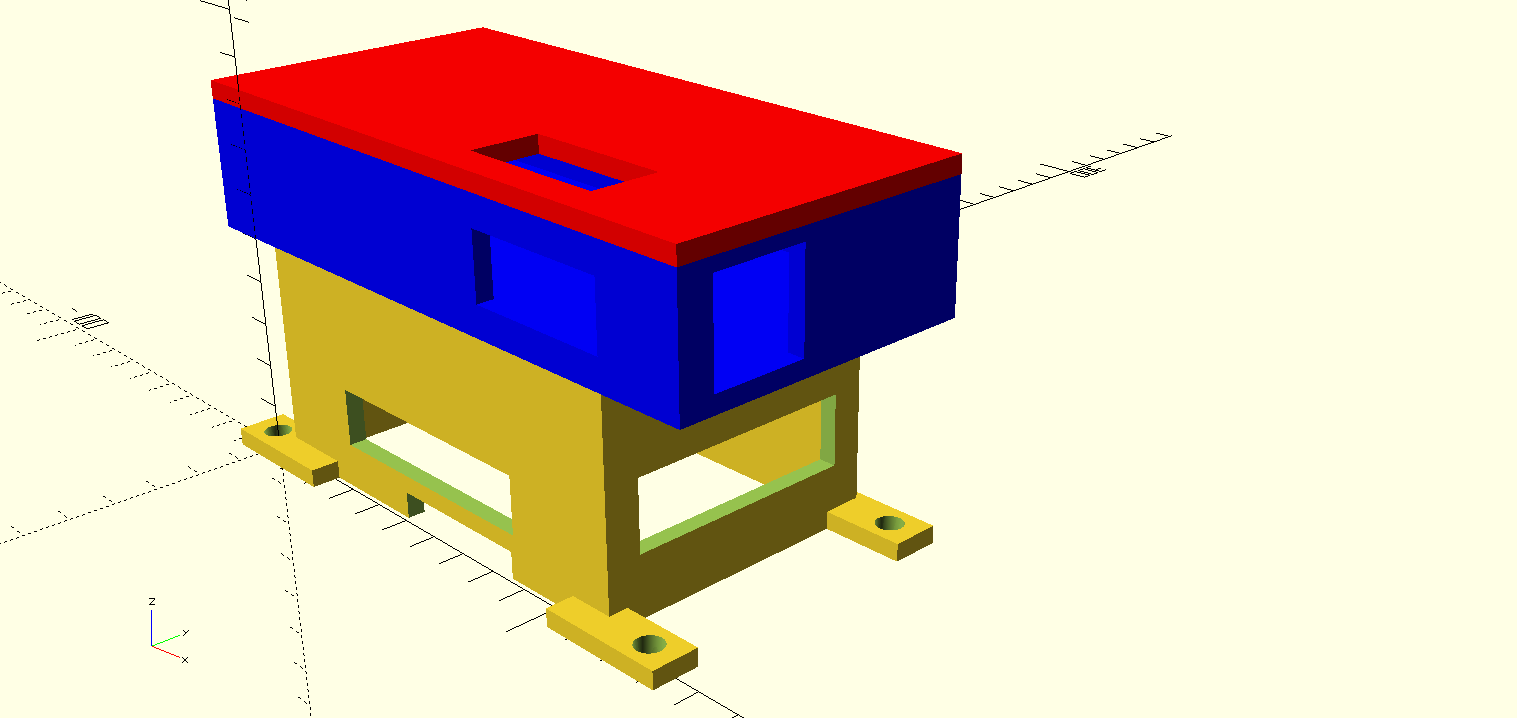
\includegraphics[scale=0.6, angle=90]{graphics/gehaeuse.png}
		\caption{Das Gehäuse in den drei Teilen}
		\label{fig:case-3D}
\end{figure}

\newpage
\subsection{Gehäuse - Kunststoffwerkstätte}

Als Alternativlösung wird das Gehäuse in der Kunststoffwerkstätte gefertigt. Dieses soll aus poliertem weißem Kunststoff bestehen. \\
Dazu soll noch eine Ladebuchse und ein Schalter verbaut werden. \\
Nach Absprache mit Fachlehrer Strohmaier, welcher mich hier Tatkräftig unterstützt hat, wurde das Gehäuse in folgenden Schritten produziert:
\begin{itemize}
	\item{Die Bodenplatte und die beiden Seitenteile werden aus weißem Kunststoff heraus geschnitten}
	\item{Die Bodenplatte wird gebogen und mit den beiden Seitenteilen verklebt}
	\item{Es werden vier Löcher als Befestigungsschrauben gebohrt}
	\item{Die Platte für den Bildschirm wird Ausgeschnitten und die Versenkung für den Bildschirm hineingefräßt}
	\item{Die Abstandshalter (innen) werden ausgeschnitten und in beide werden Löcher für die Schrauben gebohrt}
	\item{Die Löcher für die Mikro-USB-Buchse und für den Ein-Ausschalter wird hineingeschnitten (Lasercutter)}
	\item{Es werden Schrauben für das verschließen des Displays gesucht. Da es keine >50mm langen M3 Schrauben gibt, wird eine Gewindestange abgeschnitten und das Gehäuse mit einer Mutter befestigt.}
	\item{Damit die Mutter nicht gesehen wird, werden vier Standfüße besorgt in denen die Mutter platz hat.}
\end{itemize}

%TODO BILD

%=================================================================================
\clearpage\vfill\newpage{}
%=================================================================================
\section{Android}
\label{SEC:android}


%=================================================================================
\clearpage\vfill\newpage{}
%=================================================================================
\section{\sc Fertigungsdokumentation}
	{\yhbu
	Die Fertigungsdokumentation ist als optionaler Dokumentationsteil zu sehen und
	wird mit der Betreuerin bzw. Betreuer besprochen, ob dieser Teil der Dokumentation
	notwendig ist. Gedacht ist die Fertigungsdokumentation speziell für aufwändige
	Schaltungen, bei denen es notwendig erscheint, einen Verkabelungsplan, spezielle
	Anleitungen für das Einlöten der Bauteile usw. auszuarbeiten.
	}
\section{\sc Benutzerdokumentation}
	{\yhbu
	Hinweis: Die Benutzerdokumentation beschreibt das System aus der Sicht des
	Benutzers. Ein beliebiger Benutzer sollte in die Lage versetzt werden, das System
	zu verwenden (Bedienungsanleitung, technische Dokumentation).
	}
 \subsection{Installationsanleitung}
	{\yhbu
	Schritt-für-Schritt-Anleitung, wie das System vom Benutzer erstmalig in Betrieb
	genommen werden kann. Weiters eine Anleitung, wie die Software des Systems mit
	Hilfe der Entwicklungswerkzeuge neu erstellt werden kann.
	}
 \subsection{Anwendungsbeispiele}
	{\yhbu
	Beschreibung typischer Aufgaben, die der Benutzer mit dem System durchführen
	kann (Schritt-für-Schritt-Anleitungen).
	}
 \subsection{Referenzhandbuch}
	{\yhbu
	Beschreibung der einzelnen Bedienungselemente (Frontplatten, Dialoge...).
	}
 \subsection{Fehlermeldungen und Hinweise auf Fehlerursachen}
	{\yhbu
	Alle Fehlermeldungen, die das System dem Benutzer ausgeben kann, mit
	Beschreibung der Ursache und Vorschlägen zur Lösung des Problems.
	}









%=================================================================================
\clearpage\vfill\newpage{}
%=================================================================================
\renewcommand{\thepage}{\Roman{page}}% Roman for page counter
\setcounter{page}{1}
\renewcommand{\thesection}{\Roman{section}\;}
%\renewcommand{\labelsection}{(\roman{section})}
\setcounter{section}{0}
%\section{\sc \;}\hfill\\[-24mm]
	%Abbildung 2: Zeitplanung Projekt	8
\section{Abbildungsverzeichnis}\noindent%
\begingroup
\renewcommand{\section}[2]{}
	\listoffigures
\endgroup

%\section{\sc \;}\hfill\\[-23mm]
	%Tabelle 1: Arbeitsaufstellung	9
\section{\sc Tabellenverzeichnis}\noindent%
\begingroup
\renewcommand{\section}[2]{}	
	\listoftables
\endgroup









%=================================================================================
\clearpage\vfill\newpage{}
%=================================================================================
%\renewcommand{\thepage}{\rom{page}}% Roman for page counter
\renewcommand{\thesection}{\Roman{section}\;}
\setcounter{section}{2}
%\vspace*{-8mm}
\section{Literaturverzeichnis}
\cmnt{
	{\yhbu
	Beispiele:
	\\[0mm]{\fontsize{10pt}{10pt}\selectfont
	(Übernommen aus dem Leitfaden des BMBF Reife- und Diplomprüfungen März 2014)
	\\[0mm]
	\begin{description*}
	\item[1. Werke eines Autors] Nachname, Vorname: Titel. Untertitel. -
		Verlagsort: Verlag, Jahr. Nachname,
		Vorname: Titel. Untertitel. Auflage - Verlagsort: Verlag, Jahr.
		\\[1mm]Beispiele:
		\\Sandgruber, Roman: Bittersüße Genüsse. Kulturgeschichte der Genußmittel. – Wien:
		Böhlau, 1986. Messmer, Hans-Peter: PC-Hardwarebuch. Aufbau, Funktionsweise,
		Programmierung. Ein Handbuch nicht nur für Profis. 2. Aufl. - Bonn: Addison-Wesley,
		1993.
		\vspace*{2mm}
	\item[2. Werke mehrerer Autoren] Nachname, Vorname; Nachname, Vorname; Nachname, Vorname: Titel.
		Untertitel. Auflage - Verlagsort: Verlag, Jahr.
		\\[1mm]Beispiel:
		\\Bauer, Leonhard; Matis, Herbert: Geburt der Neuzeit. Vom Feudalsystem zur
		Marktgesellschaft. - Mün- chen: Deutscher Taschenbuch Verlag, 1988.
		\vspace*{2mm}
	\item[3. Sammelwerke, Anthologien, CD-ROM mit Herausgeber] Nachname, Vorname (Herausgeber):
		Titel. Untertitel. Auflage - Verlagsort: Verlag, Jahr. Nachname, Vorname: Titel.
		Untertitel. In: Nachname, Vorname (Herausgeber): Titel. Untertitel. Auflage -
		Verlagsort: Verlag, Jahr.
		\\[1mm]Beispiele:
		\\Popp, Georg (Hg.): Die Großen der Welt. Von Echnaton bis Gutenberg. 3. Aufl. -
		Würzburg: Arena, 1979. Killik, John R.: Die industrielle Revolution in den Vereinigten
		Staaten. In: Adams, Willi Paul (Hg.): Die Vereinigten Staaten von Amerika. Fischer
		Weltgeschichte Bd. 30. - Frankfurt am Main: Fischer Taschenbuch Verlag, 1977. Killy,
		Walther (Hg.): Literatur Lexikon. Autoren u. Werke deutscher Sprache. – München:
		Bertelsmann, 1999. (Digitale Bibliothek, 2)
		\vspace*{2mm}
	\item[4. Mehrbändige Werke] Nachname, Vorname: Titel. Bd. 3 - Verlagsort: Verlag, Jahr.
		\\[1mm]Beispiel:
		\\Zenk, Andreas: Leitfaden für Novell NetWare. Grundlagen und Installation. Bd. 1 - Bonn:
		Addison Wesley, 1990.
		\vspace*{2mm}
	\item[5. Beiträge in Fachzeitschriften, Zeitungen] Nachname, Vorname des Autors des bearbeiteten
		Artikels: Titel des Artikels. In: Titel der Zeitschrift, Heftnummer, Jahrgang, Seite
		(eventuell: Verlagsort, Verlag).
		\\[1mm]Beispiel:
		\\Beck, Josef: Vorbild Gehirn. Neuronale Netze in der Anwendung. In: Chip, Nr. 7, 1993,
		Seite 26. - Würzburg: Vogel Verlag.
		\vspace*{2mm}
	\item[6. CD-ROM-Lexika]\hfill
		\\[1mm]Beispiel:
		\\Encarta 2000 - Microsoft 1999.
		\vspace*{2mm}
	\item[7. Internet] Nachname, Vorname des Autors: Titel. Online in Internet: URL: www-Adresse, Datum.
		(Autor und Titel wenn vorhanden, Online in Internet: URL: www-Adresse, Datum auf
		jeden Fall)
		\\[1mm]Beispiel:
		\\Ben Salah, Soia: Religiöser Fundamentalismus in Algerien. Online im Internet:
		URL: >>http:/\slash{}www.hausarbeiten.de\slash{}cgi-bin\slash{}superRD.pl<<,
		22.11.2000. Der Weg zur Doppelmonarchie.
		Online in Internet: URL:
		http:/\slash{}www.parlinkom.gv.at\slash{}pd\slash{}doep\slash{}d-k1-2.htm,
		22.11.2000.
		\vspace*{2mm}
	\item[8. Firmenbroschüren, CD-ROM] Werden Inhalte von Firmenunterlagen verwendet,
		dann ist ebenfalls die Quelle anzugeben.
		\\[1mm]Beispiel:
		\\Digitale Turbinenregler. Broschüre der Firma VOITH-HYDRO GmbH, 2012.
		\vspace*{2mm}
	\item[9. Abbildungen, Pläne] Werden Abbildungen aus einer fremden Quelle
		[z.B. Download, Scannen) in die Diplomarbeit eingefügt,
		so ist unmittelbar darunter die Quelle anzugeben.
		\\[1mm]Beispiel:
		\\Abb. 1: Digitaler Turbinenregler [ANDRITZ HYDRO]
		\vspace*{2mm}
	\item[10. Persönliche Mitteilungen]\hfill
		\\[1mm]Beispiel:
		\\Persönliche Mitteilung durch: König, Manfred:
		Kössler GmbH Turbinenbau am 8. März 2013.
	\item[]{The RaspberryPI Foundation: Power Supply. Online im Internet: }
	\item[2.Akkumulatortypen]{
 	}
	\end{description*}
	}}%yhbu
	}

\begingroup
\renewcommand{\section}[2]{}
\begin{thebibliography}{}
\bibitem{wiki:chess}
    Author = "Wikipedia contributors",
    Titel = "Chess --- Wikipedia{,} The Free Encyclopedia",
    Jahr = "2018",
    URL = "\url{https://en.wikipedia.org/w/index.php?title=Chess&oldid=829981577}",
    Notiz = "[Online; accessed 19-March-2018]"
    
    \bibitem{SkyNet}
    	Author = Mike Klein, Titel = Google's AlphaZero Destroys Stockfish in 100-Game Match, 
    	URL = \url{https://www.chess.com/news/view/google-s-alphazero-destroys-stockfish-in-100-game-match}
	
	\bibitem{SquareTables}
	Author = ,,Abarent'', Titel = Piece Square Table, URL = \url{http://www.chessbin.com/post/Piece-Square-Table}    	
	
	\bibitem{RaspiSpecs}
	Author = The MagPi Magazine, Titel = RASPBERRY PI 3 IS OUT NOW! SPECS, BENCHMARKS \& MORE, 
	UTL = \url{https://www.raspberrypi.org/magpi/raspberry-pi-3-specs-benchmarks/}
	
	\bibitem{RaspiScreen}
	Author = ,,Gordon'', Titel = THE EAGERLY AWAITED RASPBERRY PI DISPLAY, 
	URL = \url{https://www.raspberrypi.org/blog/the-eagerly-awaited-raspberry-pi-display/}
    	
	\bibitem{RaspiPower}
		Author: The RaspberryPI Foundation, Titel: Power Supply,
		URL:\url{https://www.raspberrypi.org/documentation/hardware/raspberrypi/power/README.md},
		Notiz = Online; Stand 19. März 2018
		
	\bibitem{wiki:akku}
	 Author = "Wikipedia",
   Titel = ,,Akkumulator --- Wikipedia{,} Die freie Enzyklopädie'',
   Jahr = "2018",
   URL = "\url{https://de.wikipedia.org/w/index.php?title=Akkumulator&oldid=175107886}",
   Notiz = "[Online; Stand 19. März 2018]"
   
   \bibitem{akku-liion}
   Author = RS-Components,
   Titel = Ansmann Lithium-Akkupacks 3.7V/2600mAh, mit Drahtanschluss,
   URL = \url{https://at.rs-online.com/web/p/lithium-akkus/7760853/?searchTerm=776-0853},
	Notiz = Online; Stand 19. März 2018,
	RS-Best. Nr.: 776-0853,
	Herst. Teile-Nr.: 2347-3003
	
	\bibitem{akku-lipo}
	Author = RS-Components,
	Titel = RS Pro Li-Po Akku 3.7V, 2000 mAh, mit Drahtanschluss,
	URL = \url{https://at.rs-online.com/web/c/batterien/akkus/lithium-akkus/?applied-dimensions=4294830943},
	Notiz = Online; Stand 19.März 2018,
	RS-Best Nr.: 125-1266
	\bibitem{LM2596} 
	Komponente: LM2596
	
	\bibitem{LT1370}
	Komponente: LT1370
	
	\bibitem{Powerbank}
	Komponente=Powerbank,\\
	URL= \url{https://www.ravpower.com/support/product/manual/view/MjY5}
	
\end{thebibliography}
\endgroup


%=================================================================================
\clearpage\vfill\newpage{}
%=================================================================================
\renewcommand{\thesection}{\Roman{section}\;}
\setcounter{section}{3}
\section{Abkürzungen}
\label{SEC:ACRONYMS}

\begin{acronym}[acronyms]
 \acro{GUI}{Graphical-User-Interface}
 \acro{AI}{Artificial-Intelligence}
\end{acronym}








%=================================================================================
\clearpage\vfill\newpage{}
%=================================================================================
\appendix
\part*{\sc Anhang}
\renewcommand{\thesection}{\arabic{section}\;}
\setcounter{section}{4}
\section{\sc Pflichtenheft}
\vfill
	\begin{center}\begin{huge}
			\textbf{Pflichtenheft für die Diplomarbeit}\\ \vspace{1cm}
			\textbf{JavaChess, ChessPI AndChess}
	\end{huge}\end{center}
\vfill
\newpage

\subsection{\sc JavaChess Konzept}

Das Programm ist als 2D Schachspiel konzipiert. Basierend auf Java und JavaFX wird das Spiel entwickelt. \\
Das Spiel soll Online spielbar gemacht werden, aber auch über einen Einzelspielermodus verfügen. Dieser Einzelspielermodus beinhaltet auch eine selbst entwickelte künstliche Intelligenz. \\
Die Grafische Oberfläche setzt sich aus selbst designten Schachbrett, Bedienflächen und aus Opensource-Quellen stammenden Ressourcen für die Figuren zusammen.\\
Selbstverständlich sollen alle möglichen Züge implementiert- und ein passender Schachmattalgorithmus entwickelt werden. \\
Auf eine Ressourcenschonende Zugberechnung soll besonderen Wert gelegt werden, da die künstliche Intelligenz auf denselben Zugmechanismus zugreifen soll wie der menschliche Spieler. \\
Die Bedienung des Programms soll auf mehrere Arten möglich sein:  mittels Click to Click* und Drag and Drop.\\
*Click to Click: Spieler A klickt auf Feld d7 – dann auf Feld d6 – Figur bewegt sich von d7 nach d6.

\subsection{Einzubauende Features}

\subsubsection{JavaChess (Desktop Version - Windows}

\begin{enumerate}
	\item{GUI}
	\begin{enumerate}
		\item{2D Darstellung des Schachbretts}
		\item{Bedienflächen, in Menüs geordnet}
		\item{Spielstand Indikatoren}
	\end{enumerate}
	\item{Programmlogik}
	\begin{enumerate}
		\item{Zugfunktion}
		\item{Schachmattalgorithmus}
		\begin{enumerate}
			\item{Es soll auf eine Übersichtlichkeit des Programmcodes geachtet werden}
			\item{Die Kommentare des Programmcodes sollen auf Englisch erfolgen}
		\end{enumerate}
	\end{enumerate}
	\item{Künstliche Intelligenz}
	\begin{enumerate}
		\item{Im Einzelspielermodues ist es möglich gegen eine selbst entwickelte möglich gegen eine selbst entwickelte künstliche Intelligenz zu spielen}
		\item{Die Evaluierung des besten Zuges der künstlichen Intelligenz wird mithilfe eines abgeänderten MinMax-Algorithmus erfolgen.}
	\end{enumerate}
	\item{Netzwerk}
	\begin{enumerate}
		\item{Austausch der Spieldaten über ein Local Area Network.}
	\end{enumerate}
\end{enumerate}

\subsubsection{ChessPI (Raspberry PI 3}

\begin{enumerate}
	\item{Für einen 7‘‘ Touchscreen optimierte Spielerfahrung}
	\item{Optimierung der künstlichen Intelligenz für Niedrigleistung}
	\item{Eigenentwickeltes Gehäuse, welches mithilfe eines 3D-Druckers gebaut wird}
	\item{Selber entwickelte Akkuansteuerungsschaltung und Einbau des Akkus innerhalb des Gehäuses}
\end{enumerate}

\subsubsection{AndChess (Android)}

\begin{enumerate}
	\item{Vollständig portierter Programmcode für Android basierte mobile Geräte}
	\item{Angepasste GUI für eine bessere Bedienung auf mobilen Geräten}
\end{enumerate}

\subsection{Appendix}
\subsubsection{Vorhandene Bugs}

Hier werden alle bekannten Bugs gelistet, welche behoben werden sollen:

\begin{itemize}
	\item{chachmattalgorithmus gibt außer in einem bestimmten Fall nur Schach aus.Dieser bestimmte Falls ist, wenn zwei gegnerische Figuren den König bedrohen.}
	\item{Die Züge Rochade, En Passant, Bauerntausch und der Doppelzug des Bauern, falls dieser sich noch nicht bewegt hat, sind nicht eingebaut.}
	\item{Die Züge des Läufers und der Dame haben den Fehler falls diese Diagonal ziehen, sind auch illegale Züge erlaubt. Z.B.: Lc8 -> Le6, dieser Zug funktioniert, sollte aber nicht}
	\item{Es gibt keine Feststellung ob Team1 oder Team2 am Zug ist, beide funktionieren immer.}
	\item{Falls eine Schachsituation entsteht, kann es unter besonderen Bedingungen zu einer Endlosschleife kommen. Diese lässt in Folge das Programm abstürzen.}
\end{itemize}


section{Datenblätter}
\label{SEC:DATASHEET}

\begin{figure}[H]
  \centering
		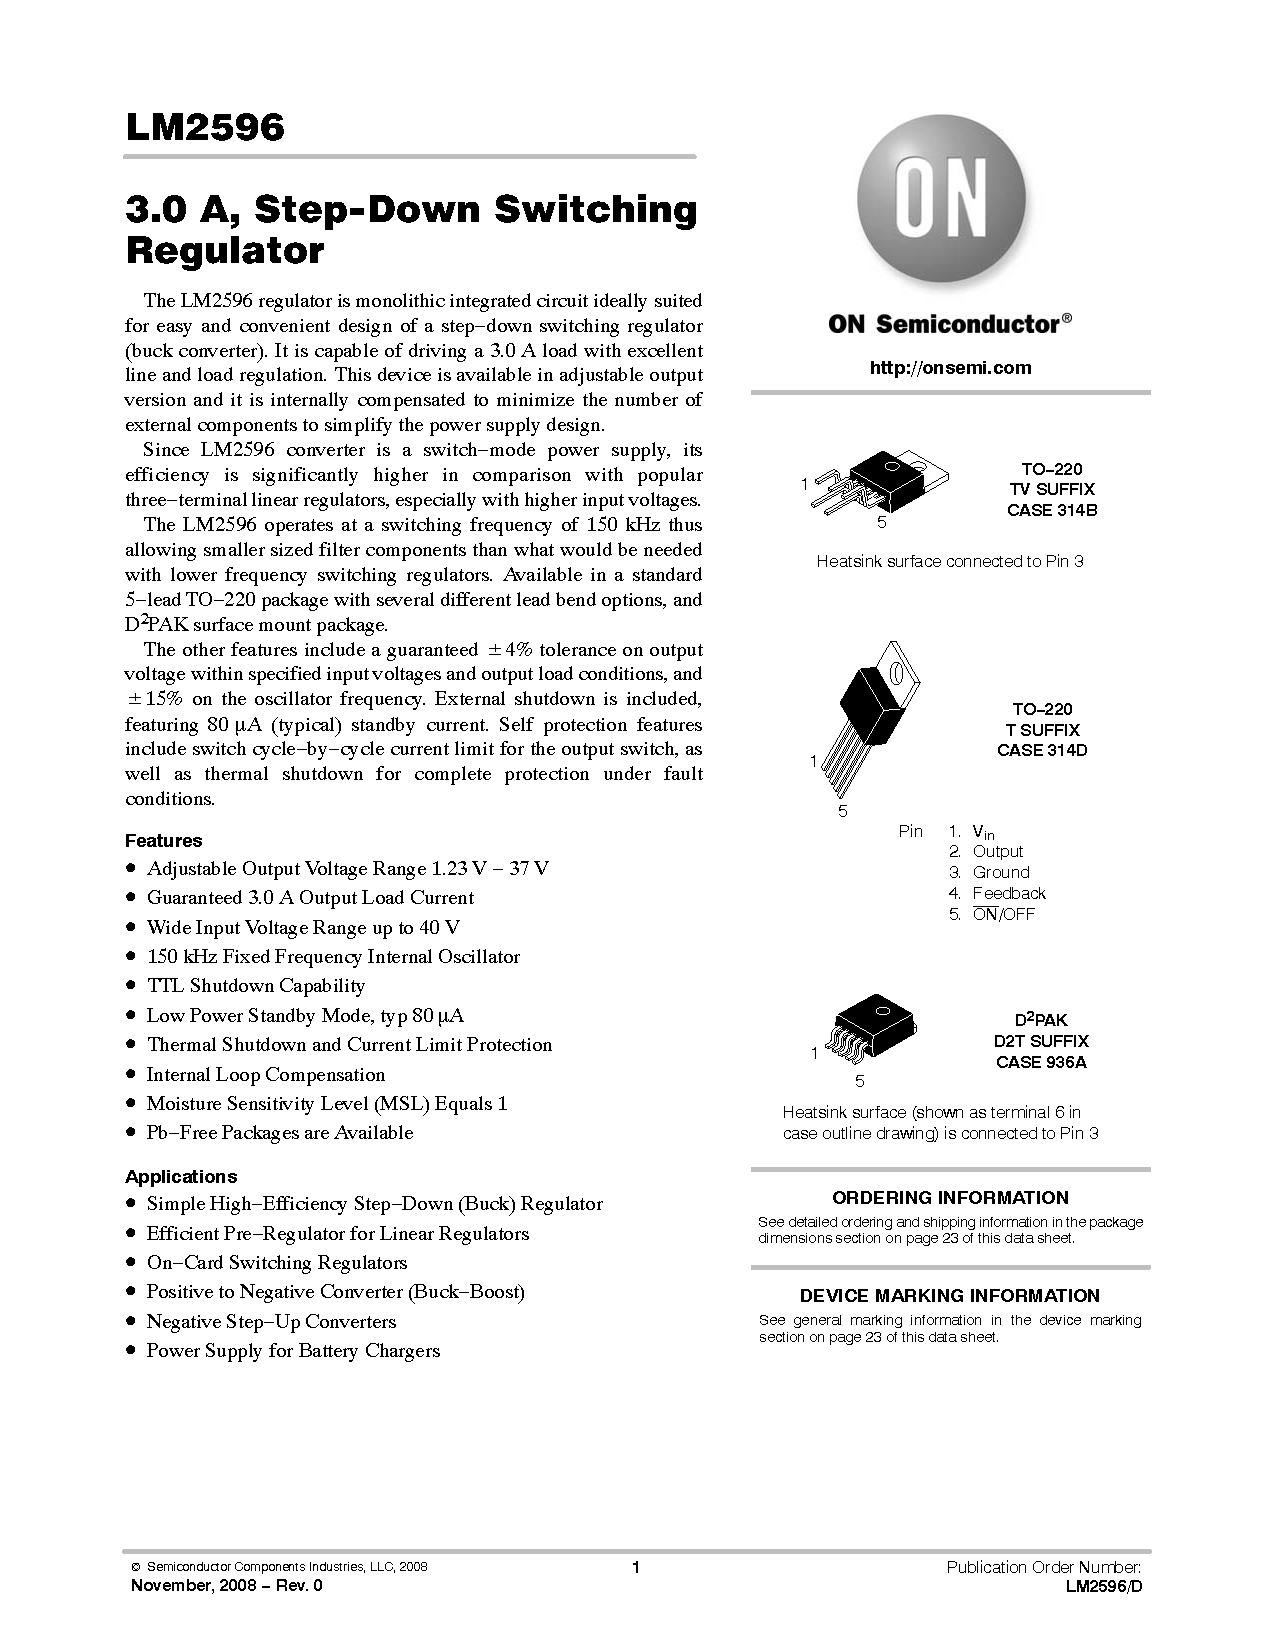
\includegraphics[scale=0.75, angle=0,page=1]{graphics/LM2596.PDF}
		\caption{Datenblatt LM2596}
		\label{datasheet:LM2596}
\end{figure}

\begin{figure}[H]
  \centering
		\includegraphics[scale=1.5, angle=90,page=2]{graphics/powerbank.pdf}
		\caption{Datenblatt Powerbank}
		\label{datasheet:powerbank}
\end{figure}

\begin{figure}[H]
  \centering
		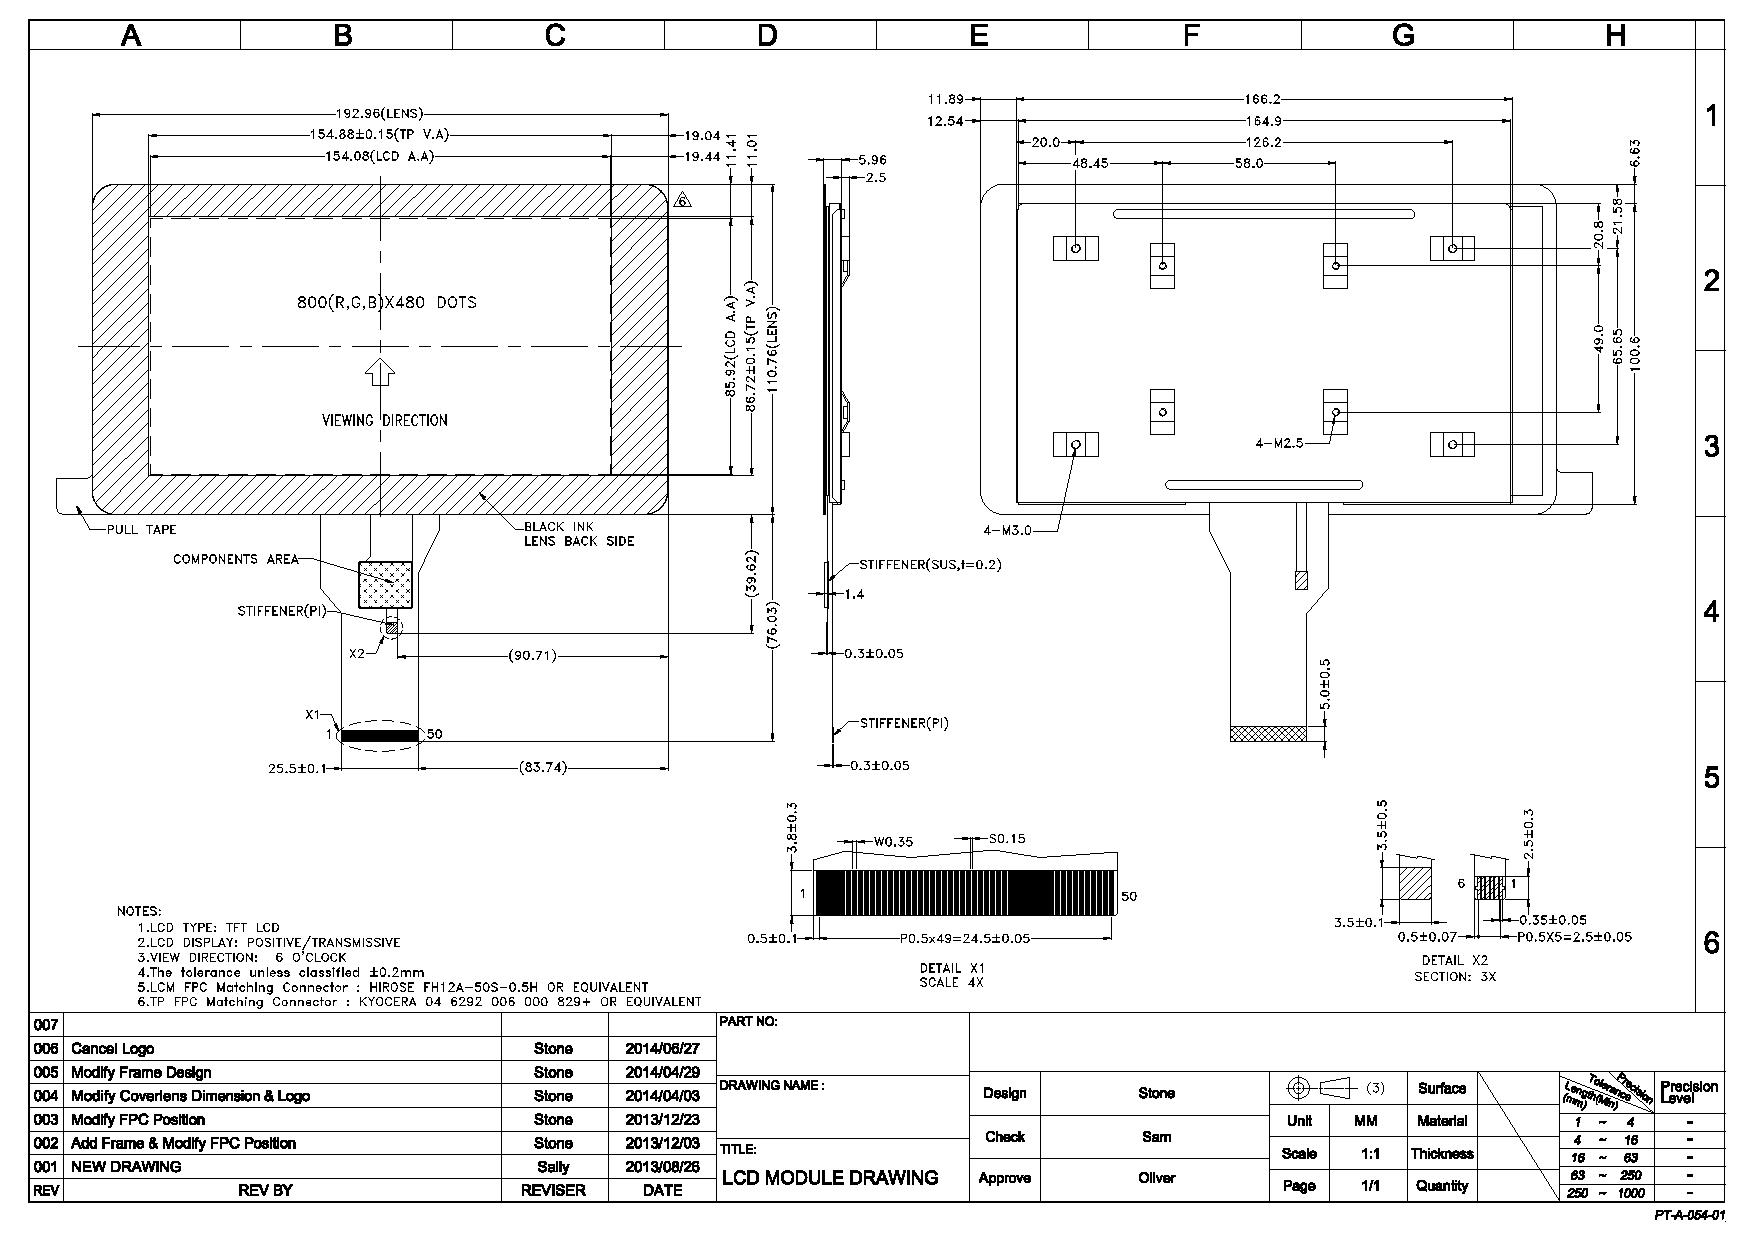
\includegraphics[scale=0.7, angle=90]{graphics/screen.pdf}
		\caption{Datenblatt RaspberryPI Bildschirm}
		\label{datasheet:raspiscreen}
\end{figure}




%==================================================================================
\clearpage\vfill\newpage
%==================================================================================
	% -???
	%iXH weiss nit, wieso da eine Leeseite zu sein hat.
	\vfill
	{\color{white} NIX}




%==================================================================================
\clearpage\vfill\newpage
%==================================================================================
\section{\sc Zusammenfassung}
	{\yhbu
	Kurzbeschreibung in Deutsch, eine A4-Seite.
	Die Zusammenfassung soll eine Einführung in das Thema
	der vertiefenden Aufgabenstellung geben,
	den praktischen Teil kurz beschreiben und die wichtigsten Ergebnisse
	des einzelnen Teammitgliedes anführen.
	Die Zielgruppe der Zusammenfassung sind auch Nicht-Techniker!
	}

 \subsection{Schlussfolgerung / Projekterfahrung}

 \subsection{Projektterminplanung}
	{\yhbu
	Screenshots der MS Project-Datei.
	Die Ausgabe muss lesbar sein (eventuell auf mehrere Bilder verteilen).
	Insbesondere ist darauf zu achten,
	dass die Zeitachse und die Vorgangsachse auf jedem Bild sichtbar sind!
	Es muss nicht MS-Project verwendet werden!
	\\[2mm]
	Projektbalkenplan (Gantt-Diagramm) mit Meilensteinplan:
	}
	%\fbox{\parbox{0.9\linewidth}{ \rule{0pt}{80mm} }}\hfill
	\\[2mm]
	\hspace*{12mm}
	\rule{37mm}{0pt} Abbildung 2: Projektzeitplan

 \subsection{Projektpersonalplanung und Kostenaufstellung}
	{\yhbu
	Eine Abschätzung von
	{\em Personal, Material, Fremdleistungen}
	und der damit zusammenhängenden {\em Kosten}
	ist in der Vor- bzw. Startphase zu erstellen.
	\\[1mm]
	Grundsätzlich ist die Verfügbarkeit der Ressourcen zu klären.
	ACHTUNG: Es ist zu beachten,
	dass nicht immer alle notwendigen Materialien im Lager
	und Ressourcen (zBsp. Werkstaetten)
	vorhanden bzw. frei sind.
	Die Beschaffung der Materialien ist im Zeitplan mit zu berücksichtigen.
	}
  \subsubsection{Kostenaufstellung}
	\begin{center}
	
	
		\begin{tabular}{|c|c|c|}
		\hline
		 \sc Was & \sc Wie viel &  \sc $Preis(\euro)$\\
		\specialrule{2.5pt}{1pt}{1pt}
		N-Mosfet			&		7							&		3.78				\\
		\hline
		4 Ohm Resistor	&	5 (Packung)				&		1.51				\\
		\hline
		1N5408	 			& 10 (Packung)			&		5.2		\\
		\hline
		PNP-Transistor	&	10 (Packung)			&		2.99	\\
		\hline
		R-680 $\Omega$&	10 (Packung)			&		0.26		\\
		\hline
		R-3.9k$\Omega$	& 10 (Packung)			& 0.45		\\
		\hline
		1N5821				& 50 (Packung)			&	15.25		\\
		\hline
		Akku					&	2								& 35.94				\\
			\hline
		LM348					&		10 (Packung)		& 3.34				\\
			\hline
		R-1.8 k$\Omega$& 10 (Packung)			& 0.08				\\
			\hline
		LM2596				&	1								&	3.87			\\
			\hline
		C-100$\mu$F		&	5 (Packung)				&	1.23			\\
			\hline
		L-33 $\mu$H		&	1								& 2.89				\\
			\hline
		C-220$\mu$F		&	5 (Packung)				&	0.59			\\
			\hline
		Sicherung 4A		&	10 (Packung)			&	0.73			\\
			\hline
		Raspberry 3		&	1								&	61.41			\\
			\hline
		7'' Touchscreen	&	1								&	57.7			\\
			\hline
		Micro-USB Buchse& 1									&	 20.99			\\
			\hline
		Schalter				&	1								&			12.99	\\
			\hline
		M-3-Stange			&		1							& 0.89				\\
			\hline
			USB-2.0 Kabel		&	1								&	9.99			\\
			\hline
			Mikro-USB-Verlängerung		&	1								&		9.99		\\
			\specialrule{2.5pt}{1pt}{1pt}
			\multicolumn{2}{|c|}{$\sum$} & 260.89\\
			\hline
	\end{tabular}
\end{center}

  \subsubsection{Projektkostenplan}
	{\yhbu
	Kalkulation des Gesamtprojektes:
	Personalaufwand (Kosten laut WIR3-Unterricht),
	Kosten für Hard- und Software,
	externe Kosten (z.B.: Sensoren, Bausteine, Kabelkanäle\ldots).
	}

  \subsubsection{Arbeitsnachweis Diplomarbeit}
	\label{SUBSEC:WORKDONE}	
	\cmnt{
	02.10.2017 -Alexander Beiser: Schachmatt Algorithmus und Vervollständigung des Hot-Seat Modus -Marcel Huber: Implementierung der Netzwerkfähigkeit

06.11.2017 -Alexander Beiser: Entwicklung der künstlichen Intelligenz -Marcel Huber: Implementierung von Java FX.

18.12.2017 -Alexander Beiser: Raspberry-PI Implementierung und Design des Gehäuses -Marcel Huber: Komplettüberarbeitung der GUI für eine bessere Benutzer-Erfahrung

04.02.2018 -Alexander Beiser: Entwicklung der Akku-Steuerungsschaltung und Einbau dieser -Marcel Huber: Portierung auf Android

05.03.2018 -Alexander Beiser: Durchführung einer Beta-Phase und Fehlerbehebungen -Marcel Huber: Durchführung einer Beta-Phase und Fehlerbehebungen 
		
	}
	
% Please add the following required packages to your document preamble:
% \usepackage[normalem]{ulem}
% \useunder{\uline}{\ul}{}
\begin{table}[]
\centering
\begin{tabular}{ccccc}
\multicolumn{5}{c}{\textbf{Arbeitsaufstellung}}                                                                                                                                                                                                                                  \\ \hline
\multicolumn{1}{|c|}{{\ul Was}}                                                                                                     & \multicolumn{1}{c|}{{\ul Person}} & \multicolumn{1}{c|}{{\ul Stunden}} & \multicolumn{1}{c|}{{\ul Von}}  & \multicolumn{1}{c|}{{\ul Bis}}  \\ \hline
\multicolumn{5}{|c|}{\textit{Beginn der Diplomarbeit - 14.09.2017}}                                                                                                                                                                                                              \\ \hline
\multicolumn{1}{|c|}{\begin{tabular}[c]{@{}c@{}}Schachmatt Algorithmus\\ und Hotseat Modus\end{tabular}}                            & \multicolumn{1}{c|}{Beiser}       & \multicolumn{1}{c|}{30}            & \multicolumn{1}{c|}{14.09.2017} & \multicolumn{1}{c|}{02.10.2017} \\ \hline
\multicolumn{1}{|c|}{\begin{tabular}[c]{@{}c@{}}Implementierung der \\ Netzwerkfähigkeit\end{tabular}}                              & \multicolumn{1}{c|}{Huber}        & \multicolumn{1}{c|}{35}            & \multicolumn{1}{c|}{14.09.2017} & \multicolumn{1}{c|}{02.10.2017} \\ \hline
\multicolumn{5}{|c|}{{\textit{Meilenstein 1 - 02.10.2017}}}                                                                                                                                                                                                                           \\ \hline
\multicolumn{1}{|c|}{\begin{tabular}[c]{@{}c@{}}Entwicklung der künstlichen\\ Intelligenz\end{tabular}}                             & \multicolumn{1}{c|}{Beiser}       & \multicolumn{1}{c|}{35}            & \multicolumn{1}{c|}{02.10.2017} & \multicolumn{1}{c|}{06.11.2017} \\ \hline
\multicolumn{1}{|c|}{Implementierung von JavaFX}                                                                                    & \multicolumn{1}{c|}{Huber}        & \multicolumn{1}{c|}{50}            & \multicolumn{1}{c|}{02.10.2017} & \multicolumn{1}{c|}{06.11.2017} \\ \hline
\multicolumn{5}{|c|}{{\textit{Meilenstein 2 - 06.11.2017}}}                                                                                                                                                                                                                           \\ \hline
\multicolumn{1}{|c|}{\begin{tabular}[c]{@{}c@{}}Raspberry-PI Implementierung\\ und Design des Gehäuses\end{tabular}}                & \multicolumn{1}{c|}{Beiser}       & \multicolumn{1}{c|}{45}            & \multicolumn{1}{c|}{06.11.2017} & \multicolumn{1}{c|}{18.12.2017} \\ \hline
\multicolumn{1}{|c|}{\begin{tabular}[c]{@{}c@{}}Komplettüberarbeitung der GUI\\ für eine bessere Benutzer\\ Erfahrung\end{tabular}} & \multicolumn{1}{c|}{Huber}        & \multicolumn{1}{c|}{40}            & \multicolumn{1}{c|}{06.11.2017} & \multicolumn{1}{c|}{18.12.2017} \\ \hline
\multicolumn{5}{|c|}{{\textit{Meilenstein 3 - 18.12.2017}}}                                                                                                                                                                                                                           \\ \hline
\multicolumn{1}{|c|}{\begin{tabular}[c]{@{}c@{}}Entwicklung der Akku-\\ Steuerschaltung und Einbau \\ dieser\end{tabular}}          & \multicolumn{1}{c|}{Beiser}       & \multicolumn{1}{c|}{40}            & \multicolumn{1}{c|}{18.12.2017} & \multicolumn{1}{c|}{04.02.2018} \\ \hline
\multicolumn{1}{|c|}{Portierung auf Android}                                                                                        & \multicolumn{1}{c|}{Huber}        & \multicolumn{1}{c|}{15}            & \multicolumn{1}{c|}{18.12.2017} & \multicolumn{1}{c|}{04.02.2018} \\ \hline
\multicolumn{5}{|c|}{{\textit{Meilenstein 4 - 04.02.2018}}}                                                                                                                                                                                                                           \\ \hline
\multicolumn{1}{|c|}{\begin{tabular}[c]{@{}c@{}}Durchführung einer Beta-Phase\\ und Fehlerbehebungen\end{tabular}}                  & \multicolumn{1}{c|}{Beiser}       & \multicolumn{1}{c|}{30}            & \multicolumn{1}{c|}{04.02.2018} & \multicolumn{1}{c|}{05.03.2018} \\ \hline
\multicolumn{1}{|c|}{\begin{tabular}[c]{@{}c@{}}Durchführung einer Beta-Phaseund \\ Fehlerbehebungen\end{tabular}}                  & \multicolumn{1}{c|}{Huber}        & \multicolumn{1}{c|}{40}            & \multicolumn{1}{c|}{04.02.2018} & \multicolumn{1}{c|}{05.03.2018} \\ \hline
\end{tabular}
\caption{Arbeitsaufstellung nach Meilensteine}
\label{table:workgeneral}
\end{table}

	\paragraph{\color{teal}Tabelle 1: Arbeitsaufstellung}\hfill
	{\fontsize{9pt}{9pt}\selectfont
	\\\begin{tabular}{|l|l|l|p{80mm}|l|}
	\hline
	\multicolumn{5}{|c|}{\parbox{4em}{\hfill\\[-0mm]\color{dkbu}Name}}	\\
	\hline
	Datum	&Uhrzeit	&\parbox{4em}{\hfill\\[-0mm]Stunden\\nn:nn\vspace*{1mm}}
					&Beschreibung	&Betreuer	\\
	\hline
	01.11.2004	&08:00–11:30
				& &Was wurde gemacht (eine Zeile!) &	\\
	\hline
	& & & &\\
	\hline
	& & & &\\
	\hline
	& & SUMME & &	\\
	\hline
	\end{tabular}
	}







  \subsubsection{Leistungscontrolling}
	{\yhbu
	Liefert Informationen über den Fortschritt der Projektleistungserstellung.
	Tabellarische Übersicht über alle Vorgänge: Welche Vorgänge wurden erfüllt,
	welche nicht und warum.
	}




\clearpage\vfill\newpage
	{\yhbu
	\paragraph{\em Abzugeben sind:}\hfill
	\\[1mm]2 gebundene Dokumentationen mit Deckblatt (Format: A4)
	\\[1mm]2 CDs mit allen Unterlagen (Word, Bilder, Code\ldots)
	\\[1mm]2 PowerPoint Folien im HTL Design
	(1. Folie: Vorstellung des Teams und die einzelnen Schwerpunkte
	der Kandidatinnen und Kandidaten.
	2. Folie: Überblick über das Projekt mit Fotos)
	}
	\\[4mm]
	{\yhbu
	Weiters ist vorzubereiten:
	\\[2mm]Ein PowerPoint Vortrag für die Präsentation und Diskussion
	der Diplomarbeit im HTL Design.
	Die Präsentation behandelt nur die Schwerpunkte
	der einzelnen Kandidatin und des Kandidaten.
	Die Teamleiterin\slash{}der Teamleiter gibt eine Gesamtübersicht des Projektes.
	Die Präsentation dauert maximal 8 Minuten/KandidatIn.
	}








\label{LastPage}
%\addtocontents{toc}{\protect\end{multicols}}
\end{document}





%XH 25Feb17:Anpassung gem.YH-neueVorlage 'YH-RbN1-moodle2-Vorlage_DA_sRDP_19102016.docx'
%	RbP:Logo Dicke scalable
%	RbN:Logo
%bis 21Mar17: Warten auf Modifikation Greif-Mikaelyan-Widmann (nicht erhalten)
%XH 21Mar17: Finalisierung (ohne Greif-Mikaelyan-Widmann)
%XH:RdC-1547-2213	Tests variablem '\{0.12}' in 'fancyheader'-Kopfzeilen: vergeblich
%XH:RdD:0857-1112	Text-Check2
%XH:RdF:0914-1737	Preambel-Header kommentieren+ausmisten, Abgleich m. YH'docx'-Version
